\documentclass{ijclclp}
% This template is intanted to be used with the XeLaTex compiler for supporting CJK fonts
% Title Information

\date{}
\affiliation{Netaji Subhas University of Technology, New Delhi}
%\email{\texttt{\{morris, ydc, kchen\}@iis.sinica.edu.tw}}

% Document Start
\usepackage{tikz}
\usepackage{float}
\usepackage{placeins}
\usepackage{lipsum}


\usepackage{ragged2e}
\usepackage[colorlinks=true, urlcolor=black, linkcolor=blue, citecolor=blue]{hyperref}
\usepackage{titling}
\setlength{\droptitle}{-2em}
\title {A Hybrid Deep Learning Framework for Ocular Disease Detection from Fundus Images Using LBP-Enhanced Vision Transformers and CNNs}
\author{Jiya Garg, 
Inika Agrawal, Samikshaa Bajaria
        }
        
\usepackage{longtable}
\usepackage{booktabs}
\usepackage{tabularx}
\usepackage[hyphens]{url}
\Urlmuskip=0mu plus 1mu
\def\UrlBreaks{\do\/\do-}
\usetikzlibrary{fit,backgrounds,positioning}
\usetikzlibrary{arrows.meta, positioning}
\renewcommand\thesection{\arabic{section}.}
\renewcommand\thesubsection{\arabic{section}.\arabic{subsection}.}
\renewcommand\thesubsubsection{\arabic{section}.\arabic{subsection}.\arabic{subsubsection}.}


\begin{document}
\maketitle



\thispagestyle{firstpage}
% Abstract Section
\rule{\linewidth}{0.5pt}
\begin{abstract}
\justifying
Ocular diseases such as diabetic retinopathy, glaucoma, age-related mac-
ular degeneration, and cataracts are among the leading causes of vision impairment and
blindness globally. Clinicians often face challenges in identifying these diseases early manually as it is time-consuming, subjective, and prone to errors. 
This research proposes a hybrid deep learning-based methodology for automated ocular disease detection using the ODIR dataset, which includes
5000 photos across eight distinct fundus classes characterising different ocular problems, which were classified with VGG-19, ResNet50 and vision transformer algorithms. We reformulated the multiclass classification problem into a binary cataract vs normal task to train the three models. The
models are trained with actual data as well as with images after applying Local Binary Pattern (LBP) for enhanced feature extraction on the image. The experimental results
show the superiority of combining LBP with the three models as compared to the performance of the models without LBP, with validation accuracies of 94.44\%, 100\%, and 85.71\% respectively. This approach validates the potential of combining classical feature extraction methods like LBP with deep learning for more robust and interpretable ocular disease detection.
\newline 
\\ 
\\
% Keywords Section
\textbf{Keywords:} 
Ocular disease classification, 
Fundus images, 
Deep learning, 
VGG-19, 
ResNet50, 
Vision Transformer, 
Local Binary Pattern (LBP)
\end{abstract}
\rule{\linewidth}{0.5pt}
% Sections
\section{Introduction}
\vspace*{1em}
\justifying
Healthcare systems around the world are continuously evolving to respond to the increasing prevalence of both chronic and acute diseases, whether infectious or non-infectious. As populations adopt urban lifestyles, diseases linked to poor diet, sedentary behavior and environmental factors are becoming more common. The need for early diagnosis and treatment has become more crucial, especially in regions with limited access to healthcare professionals. Technology has emerged as a transformative force in healthcare, with artificial intelligence (AI) and machine learning (ML) playing a critical role in medical diagnostics, personalized treatment planning, and healthcare accessibility~\cite{habehh2021mlhealth}.
These approaches came into the health sector domain in the 1970s, evolving from classical models like Support Vector Machine, Naïve Bayes etc. to deep learning, with increasing AI-driven innovations and investments enhancing diagnostics and healthcare solutions~\cite{guergueb2021ocular}. ML techniques have not only been able to diagnose the common diseases but are also equally capable of diagnosing the rare diseases.

Among the many medical challenges, ocular diseases present a distinct and growing threat to global public health due to their substantial impact on an individual’s quality of life. Nearly 2.2 billion people around the world experience
vision problems. The World Health Organization (WHO)
estimates that there may have been a reduction in at least
1 billion of these incidents due to emergence of new technologies~\cite{whovision2019}. Common eye diseases include glaucoma, diabetes, and
hypertension. Ocular diseases, such as diabetic retinopathy,
glaucoma, age-related macular degeneration, and cataracts 
are among the leading causes of vision impairment and
blindness globally~\cite{rahmani1996baltimore}. Although their early
detection and hence timely treatment can
lessen their impact. Common causes for ocular
diseases are age related degeneration causing cataract and vision loss, contact with certain substances, UV radiation or
injury, genetic issues, chronic health conditions like diabetes
and hypertension, infections and poor lifestyle. 

With the analysis of clinical data and prediction being digitalized, machine learning models could be utilized for the timely diagnosis and cure of ocular diseases, reducing the cost, time and risk involved in traditional approaches of diagnosing diseases~\cite{xu2023automatic, du2024recognition}. The accurate disease identification is essential and effectively. One of
the most important human organs is the eye. Primarily vision
aids in the recognition and detection of 3-dimensional objects in the surroundings. Loss of vision in one eye or both may cause a person to live an
unsettling way of life because people make decisions based
on what they observe in their daily lives. The vision loss and its impact on health can have an economic and personal impact~\cite{armstrong2014eye}.
Various eye illnesses have a variety of symptoms.
These include excruciating eye pain, an abrupt loss of vision
in one or both eyes, fuzzy vision, red eyes, and droopy
eyelids. Given the serious effects of eye problems on people,
to diagnose eye diseases, this research was done with
greater precision by using fundus images. 

This study primarily focuses on the accurate recognition of ocular diseases taking into account Local Binary Pattern (LBP)~\cite{halapathirana2023lbp} features extracted from fundus images. It aims to explore feature extraction techniques in combination with deep neural networks to effectively detect common visual disorders. By integrating texture-based features like LBP with powerful learning models, the proposed approach enhances the model’s ability to detect subtle patterns associated with different eye conditions. Fundus imaging (retinography) provides a clear view of the inside and back surface of the eye including retina, optic nerve, and blood vessels, which makes it an effective tool for visualizing the health of these structures and identifying visual abnormalities. 

Among the various ocular diseases, cataract is one of the most common and clinically identifiable conditions. The lens of the eye, which is typically transparent, becomes clouded by a cataract. Due to the distinct white film it forms in the eye, cataract is one of the easiest abnormalities to visually detect using image-based machine learning models~\cite{weni2021cataract}. In this study, the models have been trained specifically to predict cataract conditions from fundus images. This study focuses on Binary Classification(Cataract vs Normal) by leveraging Local Binary Pattern (LBP) for texture-based feature extraction in combination with deep learning models using ODIR dataset~\cite{odir5k}. 
LBP is employed to highlight local texture differences in fundus images, which are particularly effective for detecting cataract features such as lens opacity. These enhanced features are then fed into deep learning models—specifically VGG19 \cite{vggmedium,hu2024}, ResNet50 \cite{resnet50medium,resnet}, and Vision Transformer \cite{xu2023automatic,vitmedium}, each of which brings unique strengths in feature learning and generalization. This work further incorporates transfer learning, allowing the use of pre-trained models originally developed on large-scale image datasets. These models are fine-tuned for the specific task of cataract detection, resulting in reduced training time and improved performance. By combining LBP with powerful deep neural networks, our method achieves validation accuracies of over 90\% across all tested architectures, confirming the viability of texture-enhanced deep learning for medical image classification.


Hence, by utilizing ML and image-based diagnostic techniques, this research contributes to building scalable and efficient models that can assist in early-stage detection of vision-threatening ocular diseases. The \textbf{key contributions} of this study are:

\begin{itemize}
    \item A hybrid  approach for ocular disease recognition using Local Binary Pattern (LBP) features extracted from fundus images integrated with deep learning models and vision transformer.
    
    \item Emphasis on automated detection of cataract using its visual traits in fundus images.
    
    \item Comparison of multiple deep neural network (VGG-19 and ResNet50) and vision transformer architectures to optimize classification of ocular diseases.
    
    \item Utilization of transfer learning to reduce training time and improve prediction accuracy for medical imaging.
    
    \item Achievement of over 90\% accuracy in all model implementations for cataract detection.
  \end{itemize}
\vspace{0.5 em}
The rest of the paper is structured as: Section~\hyperref[sec:relwork]{ Related Work} reviews related work in ocular disease detection and deep learning techniques for medical diagnosis. Section~\hyperref[sec:method]{Methodology} consists of the details about the methodology used, including description of the ODIR dataset used for training and evaluation, preprocessing steps to standardize and augment the image data, feature extraction using LBP, and model architectures used, followed by Section~\hyperref[sec:result]{Result} which discusses the performance metrics and results obtained from various models before and after applying Local Binary Pattern technique for feature extraction.Finally, Section~\hyperref[sec:con]{Conclusion} concludes the study and outlines directions for future improvements.

\section{Related Work}\label{sec:relwork}
 \vspace{1em}
With the growing prevalence of ocular diseases such as glaucoma, cataract, and
age-related degeneration in the world, early and accurate diagnosis and treatment is crucial to pre-
vent vision loss and irreversible damage. Traditional diagnostic techniques heavily rely on ophthalmologists’ expertise, which is subjective and time-consuming, especially in resource-limited settings. Hence, as the application of machine learning to fundus imaging has become a transformative tool for automated, scalable, and high-performance diagnosis, numerous recent studies have explored different machine learning techniques and architectures for classifying ocular diseases, differing in their choice of datasets, preprocessing techniques, augmentation techniques, model architectures, training procedures and evaluation metrics. We explored a few studies dones in this context.
\newline
\newline
In a study~\cite{guergueb2021ocular}, the performances of various deep learning architectures on ODIR dataset are analyzed with EfficientNetB7 giving best results. This study processed left and right eye images independently and images were augmented using Mixup and CutMix. Focal Loss has been implemented to improve class balance. The models were trained over 100 epochs using three learning rate policies, fixed, 1cycle, and SGDR. The study reported a maximum AUC of 98.31\% and accuracy of 88.85\%. The methodology is thoughtful and incorporates a variety of techniques for data preprocessing and augmentation but still the accuracy falls a bit short as compared to other studies. Another study~\cite{ye2024ocular} is about a deep learning model DPLA-Net for classification of five ocular conditions- retinal detachment, intraocular tumors, pseudophakic subluxation syndrome, vitreous hemorrhage and normal cases, using B-scan ultrasound images. Poor resolution images were excluded before model training. While the model’s performance was exceptional as it achieved a mean classification accuracy of 94.3\% and AUC of 0.992 with good per class accuracies, it’s generalizability across datasets with images of different qualities needs to be tested. 
\newline
\newline
A 2024 study~\cite{du2024recognition} combined ResNet50 and ResNet101 for detection of eye diseases from fundus images, using transfer learning. The outputs of models trained individually  were merged using Dempster–Shafer (D-S) theory, which resulted in improvements across evaluation metrics when compared to individual models, although this fusion technique increased computational complexity. Another work~\cite{yassin2023fundus} proposed a lightweight MobileNetV2-based model to detect diabetic retinopathy (DR) from fundus images, emphasizing on architectural compactness. Fundus images were enhanced through contrast-limited adaptive histogram equalization (CLAHE). A validation accuracy of 92.1\% while maintaining a footprint of just 14 MB made it suitable for mobile devices. However, while effective for binary DR detection, its generalization ability across other diseases is unproven, and its performance dipped slightly when exposed to low-light and unbalanced datasets. 
\newline
\newline
A study~\cite{singh2024novel} introduced a hybrid feature fusion model combining handcrafted texture features with deep pre trained InceptionV3 network for glaucoma detection. The methodology involved extracting Local Binary Patterns (LBP) and Histogram of Oriented Gradients (HOG) features from optic disc regions. In parallel, fundus images were passed through a pretrained InceptionV3 network to obtain high-level deep features. These two feature streams were then concatenated and passed into a fully connected classifier.  This method outperformed standalone CNNs, achieving an accuracy of 94.7\% and AUC of 0.971. However, it also increased computational complexity and training time, and the performance was sensitive to the precise optic disc segmentation step, which indicated a dependency on preprocessing quality. 
\newline
\newline
A work~\cite{li2023cross} introduced Domain-Adaptive Adversarial Network trained on EyePACS dataset and evaluated on a different dataset Messidor. A gradient reversal layer (GRL) during training was utilized for domain-invariant feature learning, so that variations in images quality didn’t degrade performance.The model achieved an AUC of 91.2\% on the source and 88.3\% on domain, outperforming models without domain adaptation. The strength of this model lies in its cross-dataset generalizability since it was evaluated on a different dataset, though it occasionally misclassified mild cases due to overly generalized features. 
\newline
\newline
In another study~\cite{xu2023automatic}, Vision Transformers (ViT) were explored for detecting age-related macular degeneration (AMD) and other retinal disorders. The input images were split into 16×16 patches, linearly embedded and processed through stacked transformer encoder layers.This transformer-based sequential attention-driven approach achieved an accuracy of 95.1\% and  superior performance in recognizing AMD in late-stage cases. However, the model was a bit costly in terms of computational resources and training time, also occasionally suffering from overfitting in smaller datasets due to its large number of parameters. A study~\cite{prajapati2023retinal} implemented MobileNetV3 combined with quantization-aware training to deploy it on low-resource edge devices for the real-time detection of diabetic retinopathy from low-resolution fundus images. When tested on Raspberry Pi 4,it achieved real-time frame rates (15–20 fps), an accuracy of 90.2\% and latency under 100 ms. It is highly suitable for rural or remote clinics, making AI-based ocular screening accessible. Its performance dipped in identifying fine-grained features such as microaneurysms in early DR stages.
\newline
\newline
In the last study~\cite{patel2022spatial}, a stacked ensemble learning method was introduced which combined five CNN models: VGG16, ResNet101, DenseNet121, InceptionResNetV2 and EfficientNetB0. Dataset APTOS was used, and the meta-learner was Gradient Boosting Machine (GBM). This voting technique achieved an AUC of 98. 9\% and improved the F1 score by 3\% over individual models. Capturing features from each base model made it robust and accurate. However, it required high computational power and training time.
\newline
\newline
Our methodology aligns with some of the strengths of prior works, utilising pretrained architectures using transfer learning and evaluation using different metrics, but stands apart in several ways. It focuses on efficient preprocessing and model generalizability. While prior works have explored complex techniques~\cite{guergueb2021ocular} and task-specific custom networks~\cite{ye2024ocular}, our methodology differs by its simplicity while maintaining efficiency and high accuracy in binary classification tasks. We incorporated LBP preprocessing to enhance feature contrast in fundus textures which is a simple feature extraction technique and enhances the robustness of model without increasing complexity or required computational resources. Secondly, our inclusion of Vision Transformer (ViT) introduces a more recent architecture that captures global image context, providing a comparison against traditional CNNs. Lastly, our binary classification task, while narrower in scope, allowed us to fine-tune our models for high specificity for screening applications where false positives or negatives must be minimized. 
\begin{itemize}
    \item Many approaches in previous studies rely on complex architectures that require high computational resources, making them less suitable for real-time or low-resource deployments.We integrated Local Binary Pattern (LBP) as a lightweight, interpretable preprocessing step to enhance results without increasing model complexity.

    \item Many earlier works used only one deep learning model, which limited comparative insight. In contrast, our paper conducts a comparative analysis of VGG19, ResNet50, and Vision Transformer, both with and without LBP, offering a deeper performance evaluation.


  

   
\end{itemize}
Overall, our novel combination of transformer-based models and LBP-enhanced preprocessing along with pretrained CNNs like VGG19 and ResNet-50 presents a promising direction for precise, binary ocular disease detection. Future work could explore the extension of this framework to multiclass classification and the incorporation of ensemble learning strategies to further improve diagnostic robustness.
\clearpage


% \begin{table}[H]
% \small
% \centering
% \begin{tabularx}{\textwidth}{|c|c|c|X|X|}
% \hline
% \textbf{S.No.} & \textbf{Year} & \textbf{Reference} & \textbf{Idea} & \textbf{Limitation} \\
% \hline
% 1 & 2021 & [7] & Used EfficientNetB7 on ODIR dataset with Mixup and CutMix; trained with various learning rate schedules. & Accuracy still slightly lower compared to some other studies. \\
% \hline
% 2 & 2024 & [8] & Proposed DPLA-Net for 5-condition classification using B-scan ultrasound. & Needs validation across mixed image quality datasets. \\
% \hline
% 3 & 2024 & [9] & Combined ResNet50 and ResNet101 outputs using Dempster–Shafer theory. & Increased complexity and may require fine-tuning on diverse datasets. \\
% \hline
% 4 & 2023 & [6] & MobileNetV2 model with CLAHE for DR detection; suitable for mobile. & Generalizability unproven for other diseases; drops in low-light/unbalanced datasets. \\
% \hline
% 5 & 2023 & [4] & Hybrid feature fusion using LBP, HOG + InceptionV3 for glaucoma detection. & Sensitive to preprocessing and optic disc segmentation; high complexity. \\
% \hline
% 6 & 2022 & [3] & Domain-Adaptive Adversarial Network with GRL, trained on EyePACS, tested on Messidor. & Occasionally misclassifies mild cases due to over-generalization. \\
% \hline
% 7 & 2023 & [2] & Vision Transformer for AMD and retinal disorder detection via 16×16 patches. & High resource demand; prone to overfitting on small datasets. \\
% \hline
% 8 & 2023 & [20] & MobileNetV3 with quantization-aware training on Raspberry Pi for real-time DR detection. & Struggles with fine details like microaneurysms in early DR. \\
% \hline
% 9 & 2022 & [21] & Stacked ensemble (5 CNNs + GBM) for biomedical classification on APTOS. & High computational demand and long training time. \\
% \hline
% \end{tabularx}
% \caption{Summary of Recent Research Studies on Ocular Disease Detection Using Deep Learning}
% \label{tab:ocular_studies}
% \end{table}

\begin{table*}[ht]
\centering
\small
\caption{Comparative Summary of Deep Learning-Based Ocular Disease Detection Studies}
\resizebox{\textwidth}{!}{
\begin{tabular}{|p{1.8cm}|p{2.8cm}|p{2.7cm}|p{3.7cm}|p{3.7cm}|}
\hline
\textbf{Reference} & \textbf{Dataset Used} & \textbf{Preprocessing / Enhancement} & \textbf{Model / Methodology} & \textbf{Key Limitation} \\
\hline
\cite{guergueb2021ocular} & ODIR & Mixup, CutMix, Focal Loss & EfficientNetB7 with learning rate scheduling & Accuracy slightly lower than more recent methods \\
\hline
\cite{ye2024ocular} & B-scan Ultrasound & Noise filtering & DPLA-Net for 5-class classification & Needs validation on mixed-quality datasets \\
\hline
\cite{du2024recognition} & Fundus (multi-source) & Dempster–Shafer fusion strategy & ResNet50 + ResNet101 ensemble via evidence theory & Complex architecture; requires careful tuning \\
\hline
\cite{yassin2023fundus} & Fundus (DR) & CLAHE enhancement & MobileNetV2 for mobile DR detection & Limited to DR; performance dips in low-light scenarios \\
\hline
\cite{singh2024novel} & Fundus (Glaucoma) & LBP, HOG feature fusion & InceptionV3 with hybrid handcrafted-deep features & Preprocessing-sensitive; requires accurate segmentation \\
\hline
\cite{li2023cross} & EyePACS $\rightarrow$ Messidor & Domain adaptation via GRL & Domain-Adaptive Adversarial Network & Misclassifies mild cases due to overgeneralization \\
\hline
\cite{xu2023automatic} & Fundus (AMD) & 16×16 patch splitting & Vision Transformer (ViT) & Overfitting risk; high computational cost \\
\hline
\cite{prajapati2023retinal} & Low-res Fundus (DR) & Quantization-aware training & MobileNetV3 for edge deployment & Poor at capturing subtle retinal features \\
\hline
\cite{patel2022spatial} & APTOS & None specified & Ensemble of 5 CNNs + GBM meta-learner & High training time and computational load \\
\hline
\textbf{This Study} & \textbf{ODIR (Cataract vs Normal)} & \textbf{LBP-based texture enhancement} & \textbf{VGG19, ResNet50, ViT with transfer learning} & \textbf{Currently binary classification; extensible to multiclass} \\
\hline
\end{tabular}
}
\label{tab:related_work_comparison}
\end{table*}










\section{Methodology}\label{sec:method}
\justifying
In this study, we designed a pipeline to do binary classification of the fundus images into Cataract and Normal categories by using deep learning models combined with feature engineering. The key steps include dataset preparation, preprocessing and augmentation, feature extraction with Local Binary Pattern (LBP), model implementation using Transfer Learning, and performance evaluation using appropriate metrics.

\subsection{Dataset preparation}
\vspace{1em}
ODIR (Ocular Disease Intelligent Recognition) dataset from Kaggle has been used for this study \cite{odir5k}. It consists of 5,000 patients with age, color fundus photographs of left and right eyes and diagnostic keywords from doctors, obtained from multiple sources with varying resolutions, illumination and quality. The patients in this dataset are divided into eight categories of ocular diseases—Normal (N), pathological myopia (M), hypertension (H), diabetes (D), cataract (C), glaucoma (G), age-related macular degeneration (A), and other abnormalities/diseases (O). Fundus images are high-resolution photographs captured from the back of the eye using a specialized fundus camera, providing a clear view of the inside and back surface of the eye including retina, optic nerve, and blood vessels, making them effective for identifying visual abnormalities.

Figure~(\ref{fig:datadistr}) shows the distribution of ocular disease classes in the ODIR dataset. The dataset is imbalanced, with Diabetes (D), Other abnormalities (O), and Normal (N) being the most frequent categories, while diseases like Cataract (C), Glaucoma (G), and Age-related Macular Degeneration (A) have fewer samples. Figure~(\ref{fig:cvn}) specifically compares cataract and normal eye images. This study focuses only on two classes: Cataract and Normal. Using diagnostic keywords in the dataset, 594 images labeled as cataract and 509 as normal were extracted by combining both left and right eye data using Python-based filtering.
\begin{figure}
    \centering
    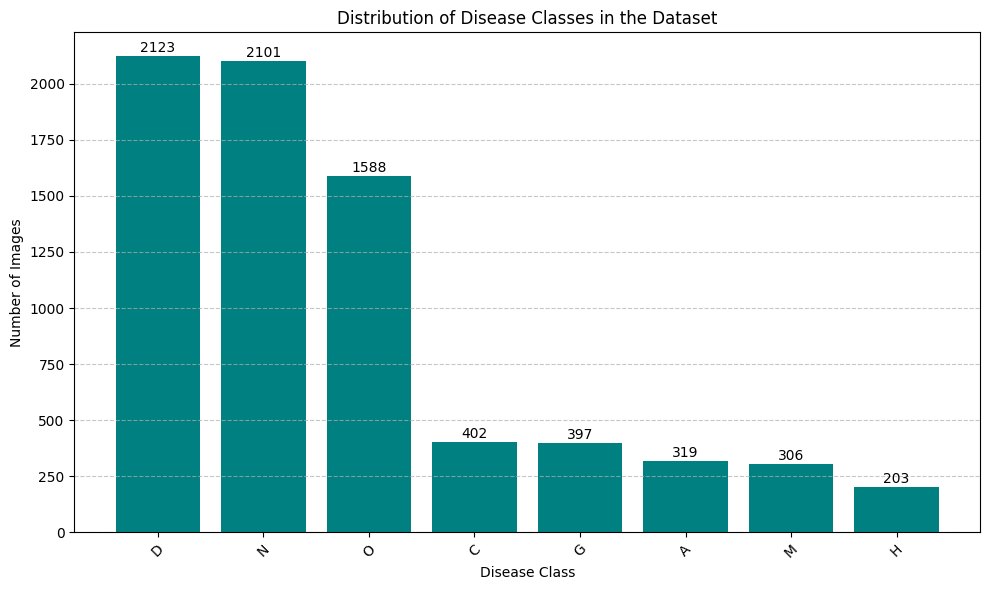
\includegraphics[width=0.7\linewidth]{image1.png}
    \caption{Distribution of Dataset}
    \label{fig:datadistr}
\end{figure}
\begin{figure}[ht]
    \centering
    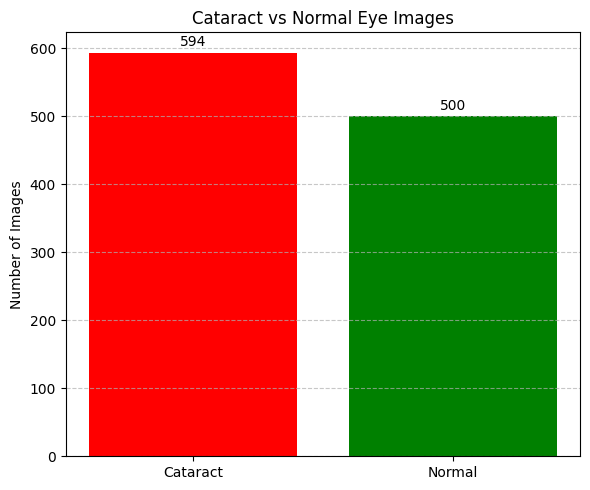
\includegraphics[width=0.6\linewidth]{image2.png}
    \caption{Cataract vs Normal eye images}
    \label{fig:cvn}
\end{figure}

The final dataset was then balanced and split into training and test sets in an 80:20 ratio.

\subsection{Image Preprocessing and Augmentation}
\vspace{1em}
Fundus images are affected by noise, blur, and inconsistent lighting due to acquisition from different sources, which may hinder effective feature extraction and reduce model performance. Hence, preprocessing was performed to improve image quality and enhance model reliability. All images were resized to 224 × 224, and pixel values were normalized to the range [0, 1]. Augmentation techniques like random rotations and zooming were applied during training to improve generalization and prevent overfitting.

\begin{enumerate}
    \item Resizing: All images were resized to 224 × 224 pixels (128 × 128 for ViT).
    \item Normalization: Pixel values were scaled to [0, 1] by dividing by 255.
    \item Augmentation: For ViT, training used random flipping, rotation, and zooming.
\end{enumerate}

\subsection{Feature Extraction using Local Binary Pattern(LBP)}
\vspace{1em}
\justifying
The texture eliminating features of the image are extracted or captured using a technique called Local Binary Pattern (LBP), which is useful to highlight disease-relevant features in fundus images. In LBP, each pixel in the image is assigned a binary value based on a comparison with the intensity values of its neighboring pixels to obtain/encode a binary pattern for the central pixel, as defined in Equation~\eqref{eq:lbp}. Uniform patterns are defined in Equation~\eqref{eq:uniform_lbp} as those that contain at most two transitions between 0 and 1 and capture essential microstructures like edges and spots. A histogram of these patterns is used to represent the frequency and regularity of different image textures, capturing essential structural information, as shown in Equations~\eqref{eq:histogram} and~\eqref{eq:normalized_histogram}. LBP has high discriminative power and computational simplicity and is robust to changes in illumination and can capture texture information in rotated and scaled images as well, making it robust while dealing with real-world medical images like fundus photographs, which may be affected with inconsistent lighting or orientation during acquisition.

In this study, LBP is used to enhance the model's ability to learn fine-grained details.LBP can facilitate improved feature learning when combined with deep learning models such as ResNet-50 and VGG19 as well as Vision Transformers. The integration of LBP extracted features can enhance the feature space with low-level texture patterns and model’s sensitivity to localized textural variations that are helpful in detecting structural abnormalities like cataract while convolutional layers in CNN models like ResNet and VGG successfully recognize high-level spatial features. Vision Transformers, which use self-attention mechanisms over image patches, can benefit from LBP's inclusion as well to concentrate on certain regions. Models' overall efficiency and accuracy in classifying eye diseases can be significantly enhanced by this hybrid approach. Figure~(\ref{fig:actualvsgrayscale}) compares an actual color image, its grayscale version, and the corresponding LBP-transformed image, showing the extracted texture patterns. Figure~(\ref{fig:imgafterlbp}) shows multiple examples of cataract and normal fundus images from the ODIR dataset after applying LBP transformation.
\begin{figure}[ht]
    \centering
    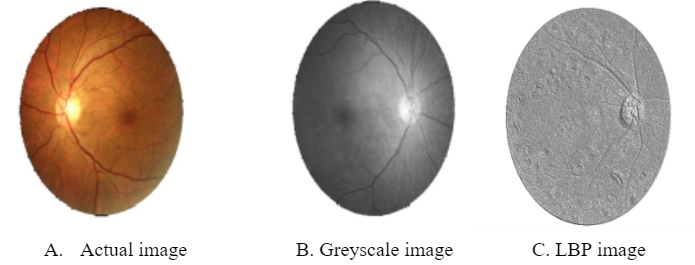
\includegraphics[width=0.64\linewidth]{image3.png}
    \caption{Comparison of raw, grayscale, and LBP-transformed fundus images}
    \label{fig:actualvsgrayscale}
\end{figure}

\begin{figure}[ht]
    \centering
    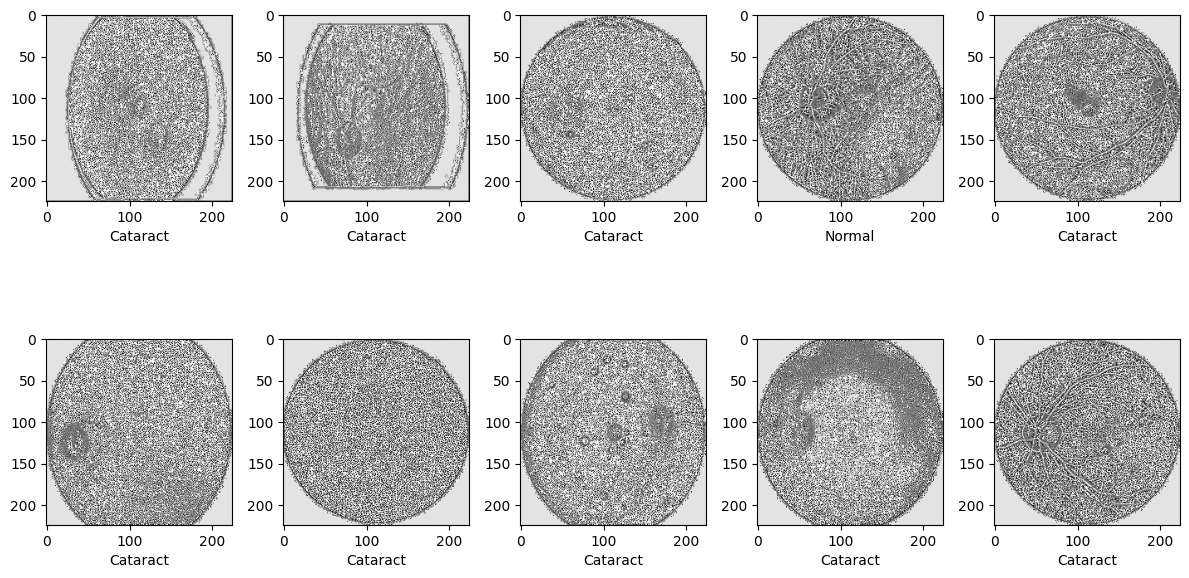
\includegraphics[width=0.71\linewidth]{image4.png}
    \caption{ODIR dataset images after applying LBP}
    \label{fig:imgafterlbp}
\end{figure}
LBP is a simple technique to effectively capture low-level structural features like edges and texture variations which are important in identifying disease-related abnormalities such as cataract-induced lens opacity. When combined with deep learning features from pretrained CNNs or Transformers, this hybrid approach improves sensitivity and specificity.
    \newline


\begin{equation}
\text{LBP}(x, y) = \sum_{p=0}^{P-1} s(I_p - I_c) \cdot 2^p
\label{eq:lbp}
\end{equation}

Where:
\begin{itemize}
  \item \( I_c = I(x, y) \): intensity of the center pixel
  \item \( I_p \): intensity of the \(p\)-th neighbor
  \item \( s(x) = 
    \begin{cases}
    1 & \text{if } x \geq 0 \\
    0 & \text{if } x < 0
    \end{cases}
  \)
\end{itemize}
Uniform patterns contain at most two transitions between 0 and 1 (or vice versa) in the binary LBP code when considered circularly.

\textbf{}
\begin{equation}
U = \sum_{p=0}^{P-1} \left| s(I_p - I_c) - s(I_{(p+1) \bmod P} - I_c) \right|
\label{eq:uniform_lbp}
\end{equation}
\newline
If \( U \leq 2 \), the pattern is considered uniform.
Uniform patterns capture essential microstructures like edges and spots. They are dominant in natural textures and reduce feature dimensionality.
\newline
Each LBP code across the image is counted to form a histogram, which represents the distribution of local texture patterns.

\textbf{}
\begin{equation}
H(k) = \sum_{x, y} \delta(\text{LBP}(x, y) - k)
\label{eq:histogram}
\end{equation}
Where \( \delta(n) = 1 \) if \( n = 0 \), otherwise \( 0 \).
To make the histogram scale-invariant, it is normalized.

\textbf{}
\begin{equation}
\hat{H}(k) = \frac{H(k)}{\sum_{j} H(j)}
\label{eq:normalized_histogram}
\end{equation}
To compare two LBP histograms, distance metrics are used.

\subsubsection*{(a) Euclidean Distance}
\begin{equation}
d(H_1, H_2) = \sqrt{ \sum_{k} \left( H_1(k) - H_2(k) \right)^2 }
\label{eq:euclidean}
\end{equation}

\subsubsection*{(b) Chi-Square Distance}
\begin{equation}
\chi^2(H_1, H_2) = \sum_{k} \frac{ \left( H_1(k) - H_2(k) \right)^2 }{ H_1(k) + H_2(k) + \epsilon }
\label{eq:chi_square}
\end{equation}
Where \( \epsilon \) is a small constant (e.g., \( 10^{-6} \)) to avoid division by zero.
\vspace{1em}

\subsection{Architectures Used}
\vspace{1em}
\subsubsection{VGG-19}
Advanced CNN—VGG19 has 19 weight layers consisting of 16 convolutions using \(3 \times 3\) filters and three fully-connected layers that have previously undergone training on the ImageNet dataset consisting of over 14 million images and 1000 classes \cite{vggmedium}. This gives it a solid understanding of shape, color, and structural aspects of an image to be used for difficult classification tasks on large-scale datasets. Its input is an image of size \(224 \times 224\) and 3 channels with its mean RGB value subtracted. It uses 5 max pooling layers of \(2 \times 2\) with stride 2. ReLU activation function is used after convolutions for introducing non-linearity. The softmax layer at the end converts the scores into class probabilities.

\begin{figure}[ht]
    \centering
    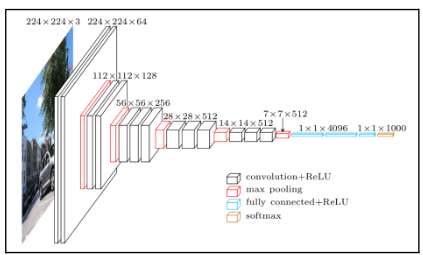
\includegraphics[width=0.65\linewidth]{image5.png}
    \caption{Architecture of VGG19}
    \label{fig:vgg19-arch}
\end{figure}
\vspace{10cm}

\vspace{1em}

\subsubsection{ResNet50}
ResNet50 is a CNN architecture consisting of 50 weight layers designed to eliminate the vanishing gradient problem by using residual learning \cite{resnet,resnet50medium}. The architecture is divided into four major parts: convolutional layers, identity block, convolutional block, and fully connected layers. Convolutional layers extract features from images and are followed by batch normalization and ReLU activation. Max pooling layers reduce dimensionality. The identity block passes the input through convolutional layers and adds it back to the output, allowing the network to learn residual features. The layers are divided into 5 stages. The key concept is the shortcut connection (skip connection), which allows the preservation of information from earlier layers. 

\begin{figure}[ht]
    \centering
    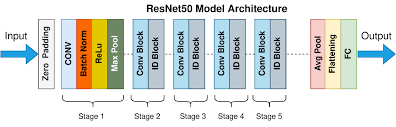
\includegraphics[width=0.65\linewidth]{image6.png}
    \caption{Architecture of ResNet50}
    \label{fig:resnet-arch}
\end{figure}



\subsubsection{Vision Transformer}
Vision Transformer (ViT) is a classification technique that employs a Transformer-like architecture \cite{xu2023automatic,vitmedium}. It partitions an image into fixed-size patches, flattens them, embeds them linearly, adds positional encodings, and feeds the resulting sequence of vectors into a standard transformer encoder. The encoder consists of multihead self-attention and feedforward layers using the GeLU activation function. ViT learns from training data to encode the relative locations of image patches to reconstruct spatial structure. The self-attention mechanism computes a weighted sum of the input data, allowing the model to give more importance to relevant features. Classification is done by appending a learnable classification token.

\begin{figure}[ht]
    \centering
    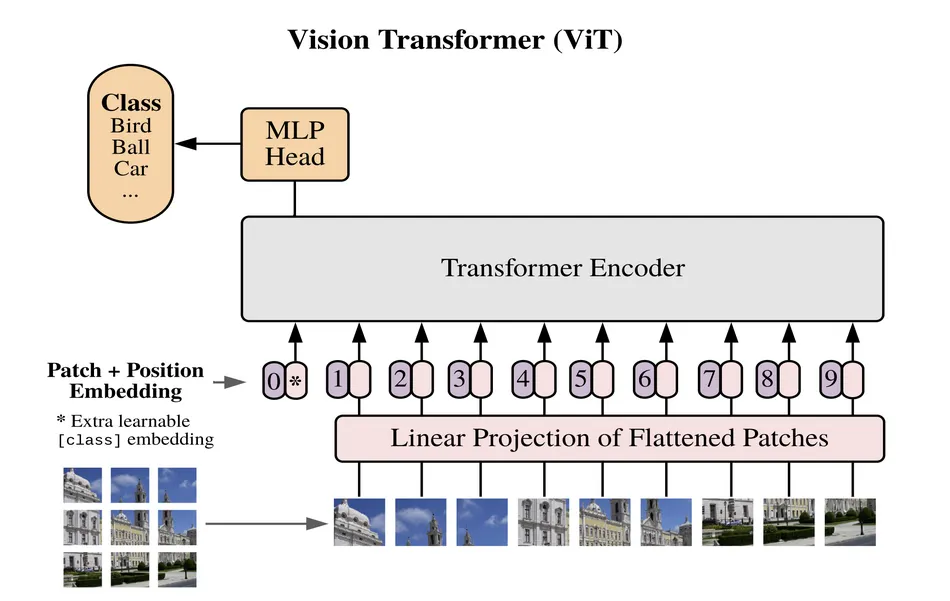
\includegraphics[width=0.6\linewidth]{image7.png}
    \caption{Architecture of Vision Transformer}
    \label{fig:vit-arch}
\end{figure}
\vspace{5cm}

\subsection{Transfer Learning-Based Model Architecture}
\vspace{1em}

Transfer Learning technique refers to the use of knowledge learnt by a pre-trained model on a large dataset (like ImageNet) for another domain-specific and smaller task. It reduces training computations and time and increases performance even with limited data. Deep learning models can be implemented more effectively using transfer learning. In this study, three pretrained models are used: VGG19, ResNet50 and Vision Transformer. Transfer learning is effective when the first model's characteristics learned on its first task are generalized and transferable to the second task, i.e., base layers are kept unchanged, reducing the number of trainable parameters and minimizing overfitting on small datasets. Fine-tuning is performed by unfreezing some of the deeper layers of the base model for domain-specific training while still benefiting from pre-trained knowledge.
\vspace{1em}
\begin{figure}[ht]
    \centering
    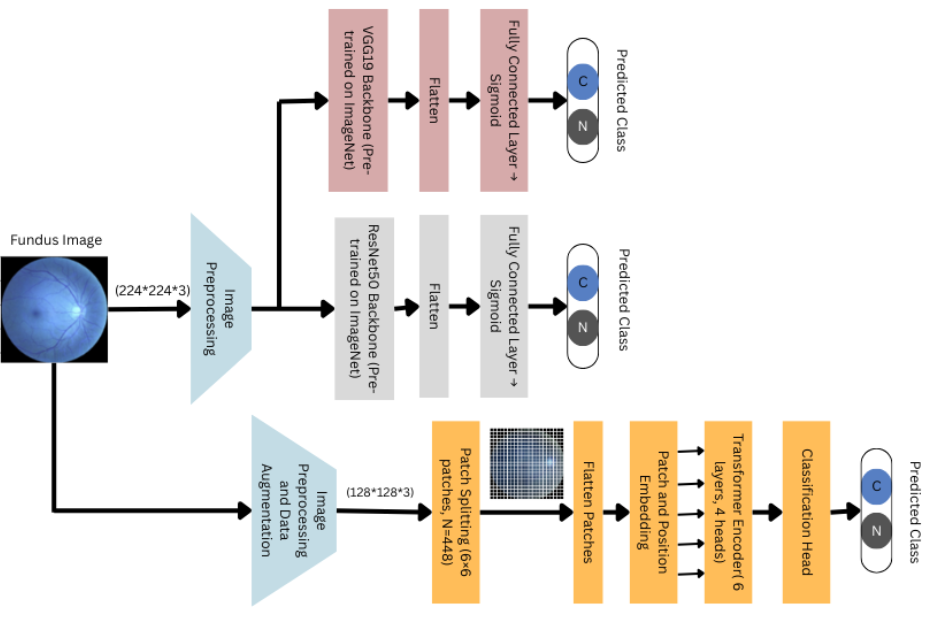
\includegraphics[width=0.95\linewidth]{image99.png}
    \caption{Architecture for cataract classification without LBP preprocessing.}
    \label{fig:arch}
\end{figure}
\subsubsection{VGG19}
A sequential model was built by appending a frozen VGG19 base \cite{vggmedium}, a global average layer to flatten and reduce dimensionality, followed by a dense fully connected layer with softmax activation(Equation~\eqref{eq:softmax_binary}) for converting scores into class probabilities for binary classification (Cataract vs Normal). The dense layer takes a single input for binary classification. Compiled using binary crossentropy loss(Equation~\eqref{eq:bce_loss}) and Adam optimizer(Equation~\eqref{eq:adam}), which adjusts the learning rate during training for convergence. EarlyStopping is a Keras callback used to stop training early if the model’s performance on the validation set stops improving, avoiding extra computation. The training stops automatically if validation accuracy doesn't improve for 5 epochs. ModelCheckpoint is another Keras callback that saves the model during training. The best-performing model according to validation accuracy is saved. 
    \newline
Softmax activation function:
    \begin{equation}
    \hat{y}_i = \frac{e^{z_i}}{e^{z_0} + e^{z_1}} \quad \text{for } i = 0, 1
    \label{eq:softmax_binary}
    \end{equation}
\newline
Binary Cross-Entropy loss:
    \begin{equation}
    \mathcal{L}_{\text{binary}} = -\frac{1}{N} \sum_{i=1}^{N} \left[y_i \log(\hat{y}_i) + (1 - y_i)\log(1 - \hat{y}_i)\right]
    \label{eq:bce_loss}
    \end{equation}
\newline
Adam Optimizer:
    \begin{equation}
    \theta_{t+1} = \theta_t - \frac{\eta}{\sqrt{\hat{v}_t} + \epsilon} \hat{m}_t
    \label{eq:adam}
    \end{equation}
\newline
Where $\eta$ is the learning rate, and $\hat{m}_t$ and $\hat{v}_t$ are bias-corrected first and second moment estimates.

    \subsubsection{ResNet50}Used the same training configuration as VGG19, leveraging residual connections for deeper network stability \cite{resnet50medium}.

    \subsubsection{Vision Transformer (ViT)}
    Input images resized to 128 × 128×3, split into patches of 6×6. The image was embedded using a custom PatchEncoder. Stacked 6 Transformer layers with 4 attention heads. Followed by a multilayer perceptron (MLP) with layers [512, 256]( Equation~\eqref{eq:mlp}). Dropout was applied between dense layers to prevent overfitting. Trained for 30 epochs using AdamW optimizer (lr=0.001, weight decay=0.0001) as defined in Equation~\eqref{eq:adamw}. Used sparse categorical loss( Equation~\eqref{eq:sparse_loss}) and checkpointed the best model \cite{xu2023automatic,vitmedium}.
\newline
Given image size \( H \times W \), and patch size \( P \times P \), number of patches:
    \begin{equation}
    N = \frac{H \cdot W}{P^2}
    \label{eq:num_patches}
    \end{equation}
\newline
Each patch is flattened and projected to a $D$-dimensional embedding space:
    \begin{equation}
    \text{PatchEmbedding} = XW_e + b_e
    \label{eq:patch_embedding}
    \end{equation}
\newline
Each layer includes Multi-Head Attention (MHA) and MLP:
    \begin{equation}
    \text{Attention}(Q, K, V) = \text{softmax}\left(\frac{QK^T}{\sqrt{d_k}}\right)V
    \label{eq:attention}
    \end{equation}
\newline
Multi-head version:
    \begin{equation}
    \text{MHA}(Q, K, V) = \text{Concat}(\text{head}_1, \dots, \text{head}_h)W^O
    \label{eq:mha}
    \end{equation}
\newline
MLP with two dense layers:
    \begin{equation}
    \text{MLP}(x) = \text{Dropout}(\text{ReLU}(xW_1 + b_1))W_2 + b_2
    \label{eq:mlp}
    \end{equation}
\newline
Sparse Categorical Cross-Entropy:
    \begin{equation}
    \mathcal{L}_{\text{sparse}} = -\frac{1}{N} \sum_{i=1}^{N} \log(\hat{y}_{i, y_i})
    \label{eq:sparse_loss}
    \end{equation}
\newline
Variant of Adam with weight decay( with weight decay coefficient \( \lambda \)) :
    \begin{equation}
    \theta_{t+1} = \theta_t - \eta \left( \frac{\hat{m}_t}{\sqrt{\hat{v}_t} + \epsilon} + \lambda \theta_t \right)
    \label{eq:adamw}
    \end{equation}
\subsection{Hybrid approach}
\vspace{1em}
        In this study, we trained two variants of each model:Without LBP( Trained on raw fundus
images) as shown in Figure~(\ref{fig:arch}) and With LBP(Trained on LBP-transformed images) as shown in Figure~(\ref{fig:lbparch}). This allowed us to compare
how texture features affect model performance when combined with deep learning. CNNs
capture hierarchical spatial features, while ViTs use attention mechanisms across image
patches. LBP complements these by enhancing local texture information.
\vspace{1em}
\begin{figure}[ht]
    \centering
    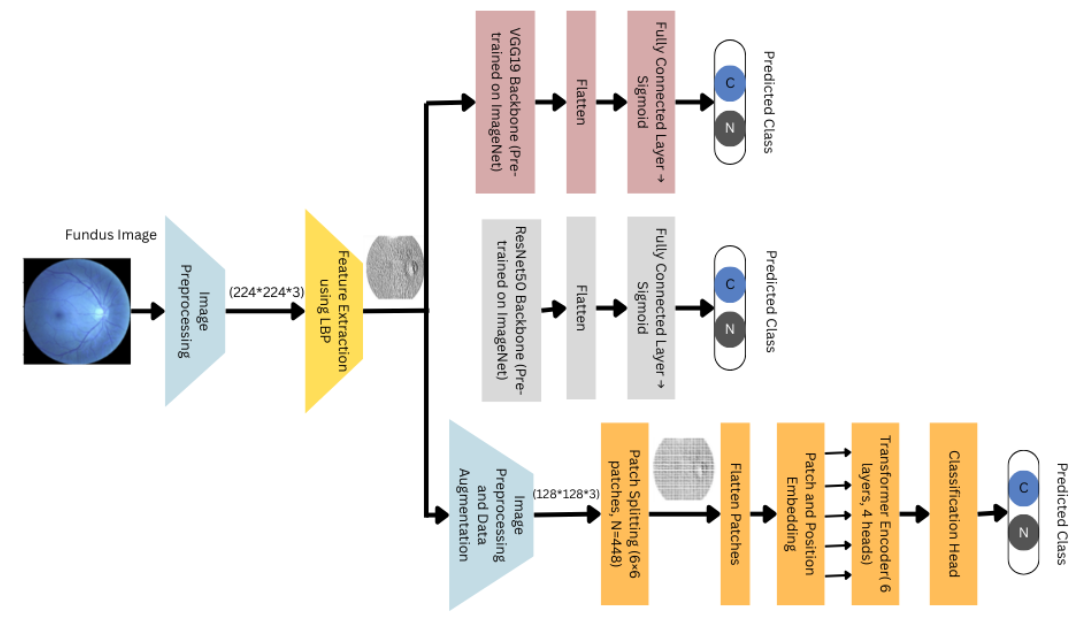
\includegraphics[width=0.95\linewidth]{image.png}
    \caption{Architecture for cataract classification with LBP enhanced preprocessing.}
    \label{fig:lbparch}
\end{figure}



\begin{figure}[h!]
\centering
\tikzstyle{startstop} = [rectangle, rounded corners, minimum width=3.5cm, minimum height=1cm,text centered, draw=black, fill=blue!20]
\tikzstyle{process} = [rectangle, minimum width=3.5cm, minimum height=1cm, text centered, draw=black, fill=orange!20]
\tikzstyle{model} = [rectangle, minimum width=3cm, minimum height=1cm, text centered, draw=black, fill=green!30]
\tikzstyle{modelt} = [rectangle, minimum width=3cm, minimum height=1cm, text centered, draw=black, fill=red!30]
\tikzstyle{evaluation} = [rectangle, minimum width=3.5cm, minimum height=1cm, text centered, draw=black, fill=gray!10]
\tikzstyle{arrow} = [thick,->,>=stealth]

\begin{tikzpicture}[node distance=2cm, scale = 0.7, transform shape]
% Start node
\node (input) [startstop] {Input ODIR Dataset\\(5000 Patients)};

% Steps
\node (segregate) [process, below of=input,text width=6cm, align=center] {Using diagnostic keywords to extract images labeled as cataract and those labeled as normal by combining both left and right eye data};
\node (resize) [process, below of=segregate,text width=6cm, align=center] {Data preprocessing: Resize Images to 224×224 and pixel values normalized to scale the intensities between 0 and 1};
\node (augment) [process, below of=resize,text width=6cm, align=center] {Apply Data Augmentation\\(Flip, Rotation, Zoom)};
\node (train) [process, below of=augment,text width=6cm, align=center] {Train Models With and Without LBP Using Transfer Learning};

% Models
\node (withoutl) [model, left=-0.1cm of train, yshift=-2cm] {Without LBP};
\node (withl) [model, right=-0.1cm of train, yshift=-2cm] {With LBP};
\node (vgg) [modelt, right=1.4cm of withoutl, yshift=-1.6cm] {VGG19};
\node (resnet) [modelt, right=1.4cm of withoutl, yshift=-3.2cm] {ResNet50};
\node (vit) [modelt, right=0.4cm of withoutl, yshift=-6cm, text width=5cm, align=center] {Vision Transformer:\\Resize images to 128×128\\Apply Data Augmentation (Flip, Rotation, Zoom)\\Extracting 6×6 patches\\GELU activation and Dropout in MLP layers};

% Arrows
\draw [arrow] (input) -- (segregate);
\draw [arrow] (segregate) -- (resize);
\draw [arrow] (resize) -- (augment);
\draw [arrow] (augment) -- (train);
\draw [arrow] (train) -- (withl);
\draw [arrow] (train) -- (withoutl);
\draw [arrow] (withl) -- (vgg);
\draw [arrow] (withl) -- (resnet);
\draw [arrow] (withl) -- (vit);
\draw [arrow] (withoutl) -- (vgg);
\draw [arrow] (withoutl) -- (resnet);
\draw [arrow] (withoutl) -- (vit);

% Border node around all components
\node[
  draw=black, 
  thick, 
  inner sep=15pt, 
  fit=(input)(segregate)(resize)(augment)(train)(withoutl)(withl)(vgg)(resnet)(vit),
  % label=below:{\parbox{0.85\linewidth}{\centering \large \textbf Proposed workflow diagram for cataract classification using the ODIR dataset. Models are trained with and without LBP preprocessing using VGG19, ResNet50, and Vision Transformer.}}
] {};
\end{tikzpicture}
\caption{Workflow for training models with and without LBP enhancement using the ODIR dataset for Cataract classification.}
\label{fig:workflow}
\end{figure}
\vspace{1em}
\begin{flushleft}
    

\subsection{Evaluation metrics}
\vspace{1em}
\justifying
        Model performance was evaluated using Accuracy(training/validation), Loss curves (training/validation), Confusion Matrix and Classification Report (Precision, Recall, F1-Score).The best-performing models (based on validation accuracy) were saved, and the metrics for all the models were compared.
        \begin{equation}
\text{Accuracy} = \frac{TP + TN}{TP + TN + FP + FN}
\label{eq:accuracy}
\end{equation}

\begin{equation}
\text{Precision} = \frac{TP}{TP + FP}
\label{eq:precision}
\end{equation}

\begin{equation}
\text{Recall} = \frac{TP}{TP + FN}
\label{eq:recall}
\end{equation}

\begin{equation}
F1 = 2 \cdot \frac{\text{Precision} \cdot \text{Recall}}{\text{Precision} + \text{Recall}}
\label{eq:f1}
\end{equation}
\newline
Where: $TP$ = True Positives, $TN$ = True Negatives, $FP$ = False Positives, $FN$ = False Negatives 


\end{flushleft}
\section{Result}\label{sec:result}
\begin{flushleft}
    \subsection{Without LBP:}
    \vspace{1em}
    \justifying
    First the models were trained and evaulated using raw fundus images without Local Binary Pattern. The three selected models, VGG19, ResNet50, and Vision Transformer were trained using transfer learning with frozen base layers and fine-tuned on the binary classification task. The performance metrics of the three models—VGG19, ResNet50, and Vision Transformer (ViT) show distinct differences in training and validation outcomes. VGG19 achieved the highest validation accuracy of 99.08\% with the lowest validation loss of 0.084891, with a training accuracy of 99.8652\% and a training loss of 0.014342, indicating strong performance and minimal overfitting. ResNet50 demonstrated perfect training accuracy at 100\% with a negligible training loss of 0.000006, but its validation accuracy was slightly lower at 97.7064\% with a validation loss of 0.131539, suggesting mild overfitting. The Vision Transformer, however, exhibited the poorest generalization, with a training accuracy of 86.3346\% and a training loss of 0.344338, while its validation accuracy was only 78.1609\% with a higher validation loss of 0.476366, highlighting significant overfitting and the weakest performance among the models.
    \end{flushleft}
\vspace{1em}
\begin{figure}[htbp]
    \centering
    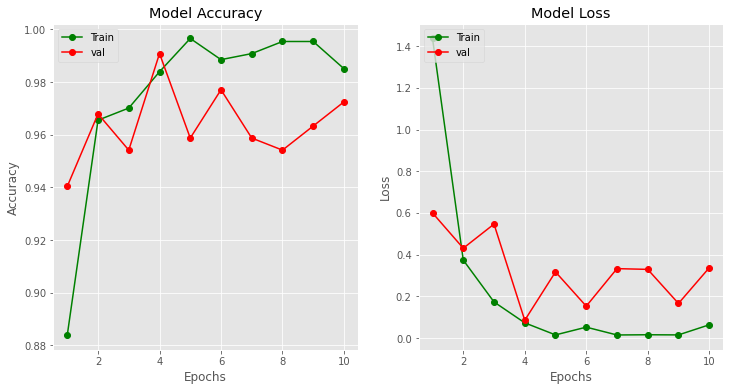
\includegraphics[width=0.70\textwidth]{image9.png}
    \caption{Training and validation accuracy/loss curves for VGG19 without LBP}
    \label{fig:vgg19_no_lbp}
\end{figure}

\begin{figure}[htbp]
    \centering
    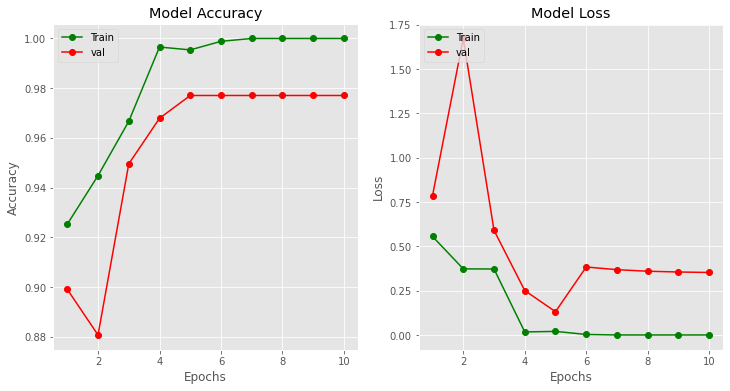
\includegraphics[width=0.70\textwidth]{image10.png}
    \caption{Training and validation accuracy/loss curves for ResNet50 without LBP}
    \label{fig:resnet50_no_lbp}
\end{figure}

\begin{figure}[htbp]
    \centering
    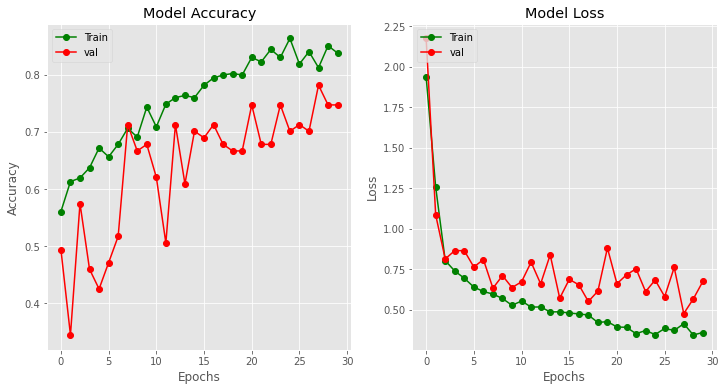
\includegraphics[width=0.70\textwidth]{image11.png}
    \caption{Training and validation accuracy/loss curves for Vision Transformer without LBP}
    \label{fig:vit_no_lbp}
\end{figure}

\begin{figure}[htbp]
    \centering
    \begin{minipage}[b]{0.48\textwidth}
    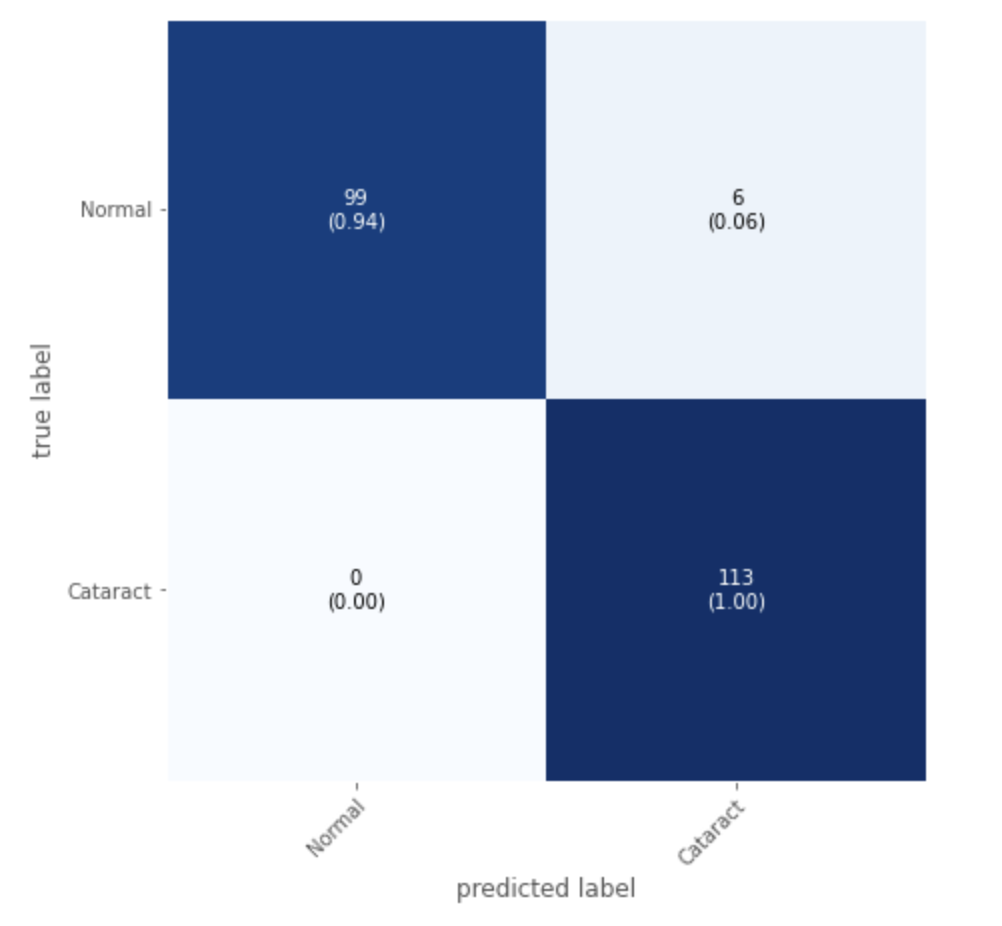
\includegraphics[width=\textwidth]{VGG.png}
    \caption{Confusion matrix of VGG19 model before LBP preprocessing}
    \end{minipage}
    \hfill
    \begin{minipage}[b]{0.48\textwidth}
    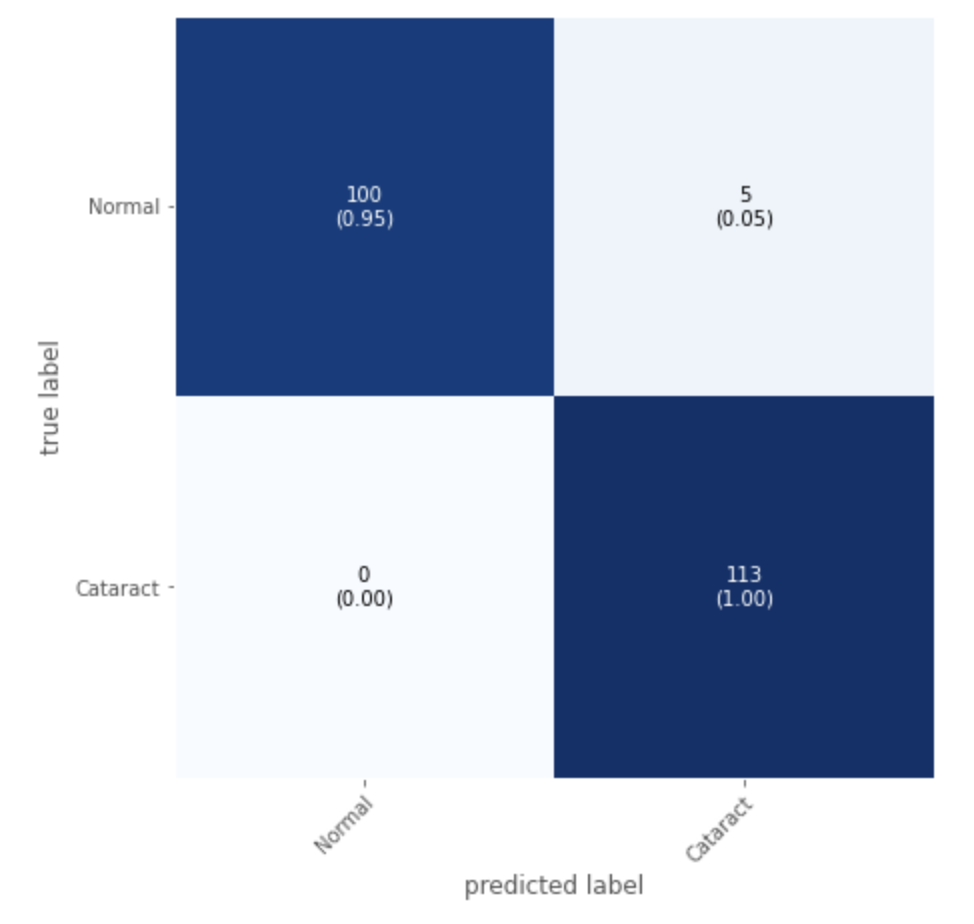
\includegraphics[width=\textwidth]{ResNet50.png}
    \caption{Confusion matrix of ResNet50 model before LBP preprocessing}
    \end{minipage}
\end{figure}
\vspace{2em}
\begin{figure}[htbp]
    \centering
    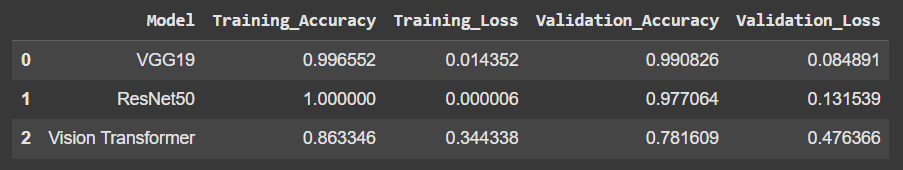
\includegraphics[width=1\textwidth]{image12.png}
    \caption{Comparison table of model metrics before LBP: VGG19 shows highest validation accuracy (99.08\%) with lowest loss (0.08), outperforming ResNet50 and Vision Transformer.}
    \label{fig:comparison_no_lbp}
\end{figure}
\vspace{2.5em}
\begin{figure}[htbp]
    \centering
    \begin{minipage}[b]{0.49\textwidth}
    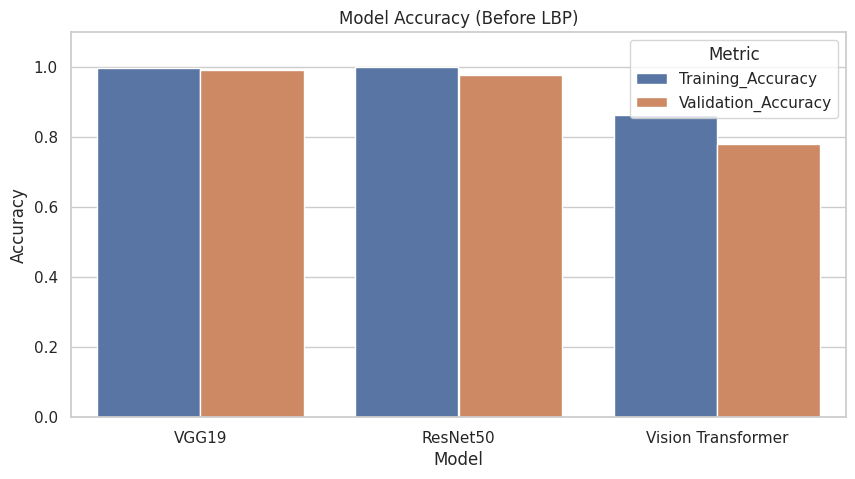
\includegraphics[width=\textwidth]{image13.png}
    \caption{Model accuracy before LBP}
    \end{minipage}
    \hfill
    \begin{minipage}[b]{0.49\textwidth}
    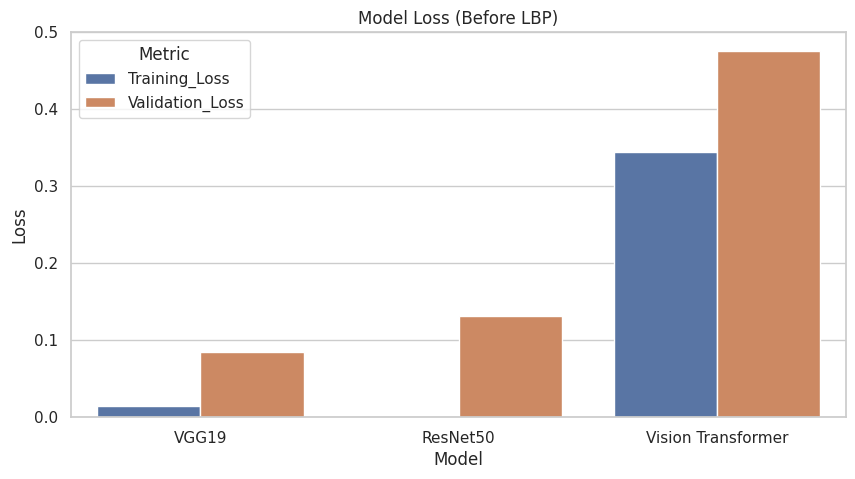
\includegraphics[width=\textwidth]{image18.png}
    \caption{Model loss before LBP}
    \end{minipage}
\end{figure}


% \vspace{10cm}

\noindent
\begin{flushleft}
\vspace{1em}
    \subsection{With LBP:}
    \vspace{1em}
    \justifying
    In the second phase, Local Binary Pattern (LBP) preprocessing was applied to all input fundus images for making structural abnormalities more distinguishable for the model and the results shifted notably. VGG19 achieved a perfect training accuracy of 100\% but with an increased training loss of 0.004897 and its validation accuracy dropped to 94.4444\% with a validation loss of 0.099631, reflecting a slight increase in overfitting. In contrast, ResNet50 showed significant improvement, with a training accuracy of 97.1014\% and a training loss of 0.046032, while achieving a perfect validation accuracy of 100\% and a reduced validation loss of 0.008169, indicating excellent generalization. The Vision Transformer also improved, with a training accuracy of 75.8065\% and a training loss of 0.746540, but its validation accuracy increased to 85.7143\% with a validation loss of 0.345332, demonstrating a substantial boost in generalization despite still lagging behind the other models in overall performance. Overall, the difference in performance before and after LBP highlights the advantage of texture-based enhancement.
\begin{figure}[htbp]
    \centering
    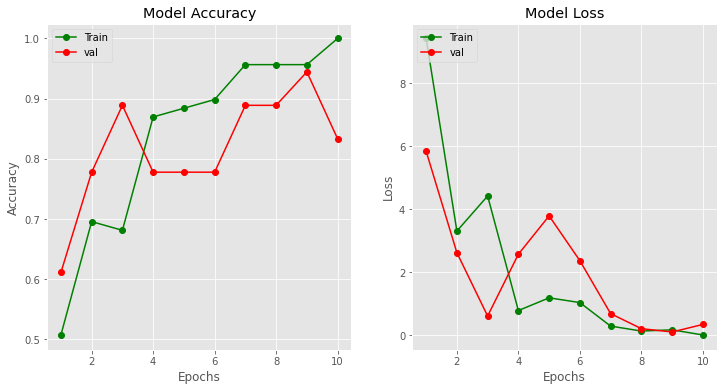
\includegraphics[width=0.70\textwidth]{image14.png}
    \caption{Training and validation accu-
racy/loss curves for VGG19 with LBP}
    \label{fig:vgg19_lbp}
\end{figure}

\begin{figure}[htbp]
    \centering
    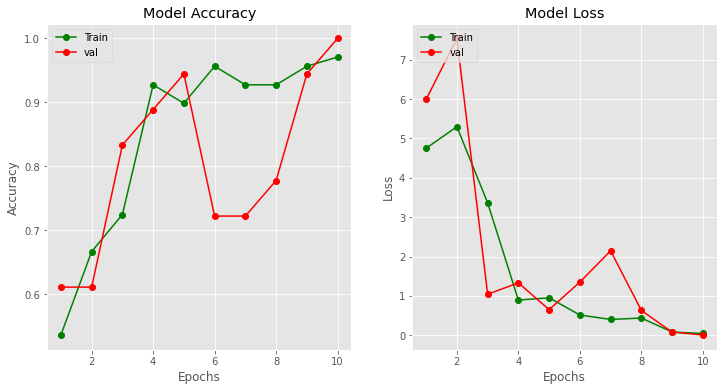
\includegraphics[width=0.7\textwidth]{image15.png}
    \caption{Training and validation accu-
racy/loss curves for ResNet50 with LBP}
    \label{fig:resnet50_lbp}
\end{figure}
\begin{figure}[htbp]
    \centering
    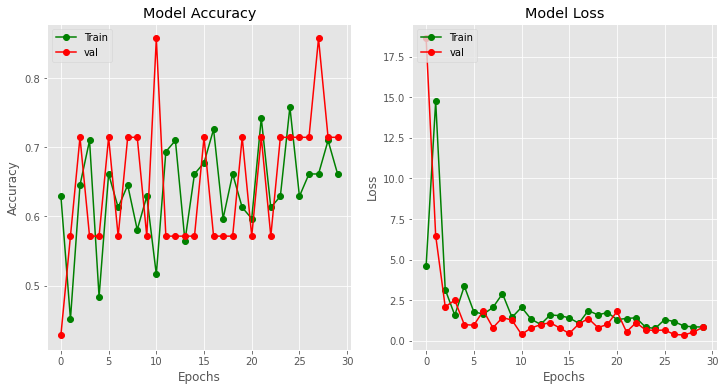
\includegraphics[width=0.7\textwidth]{image16.png}
    \caption{Training and validation accuracy/loss curves for Vision Transformer with LBP}
    \label{fig:vit_with_lbp}
\end{figure}
\noindent
\begin{figure}[htbp]
    \centering
    \begin{minipage}[b]{0.48\textwidth}
    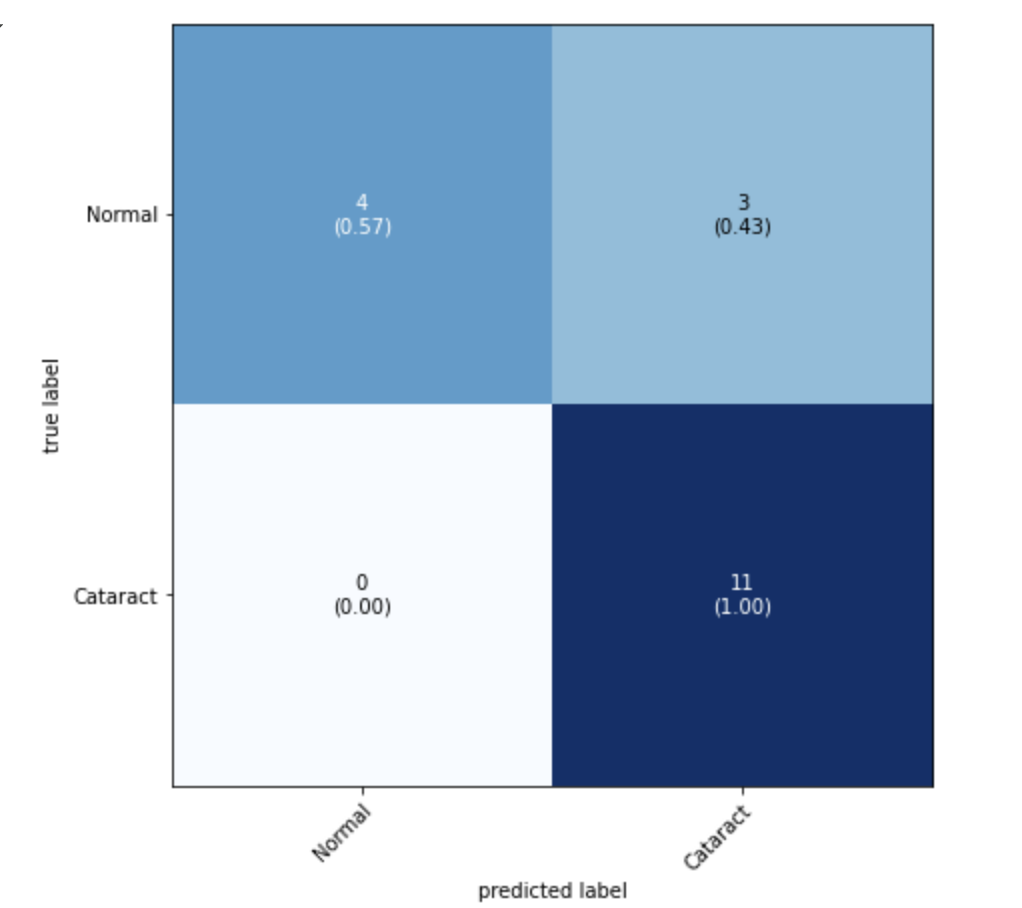
\includegraphics[width=\textwidth]{vgg19_confusion.png}
    \caption{Confusion matrix of VGG19 model after LBP preprocessing}
    \end{minipage}
    \hfill
    \begin{minipage}[b]{0.48\textwidth}
    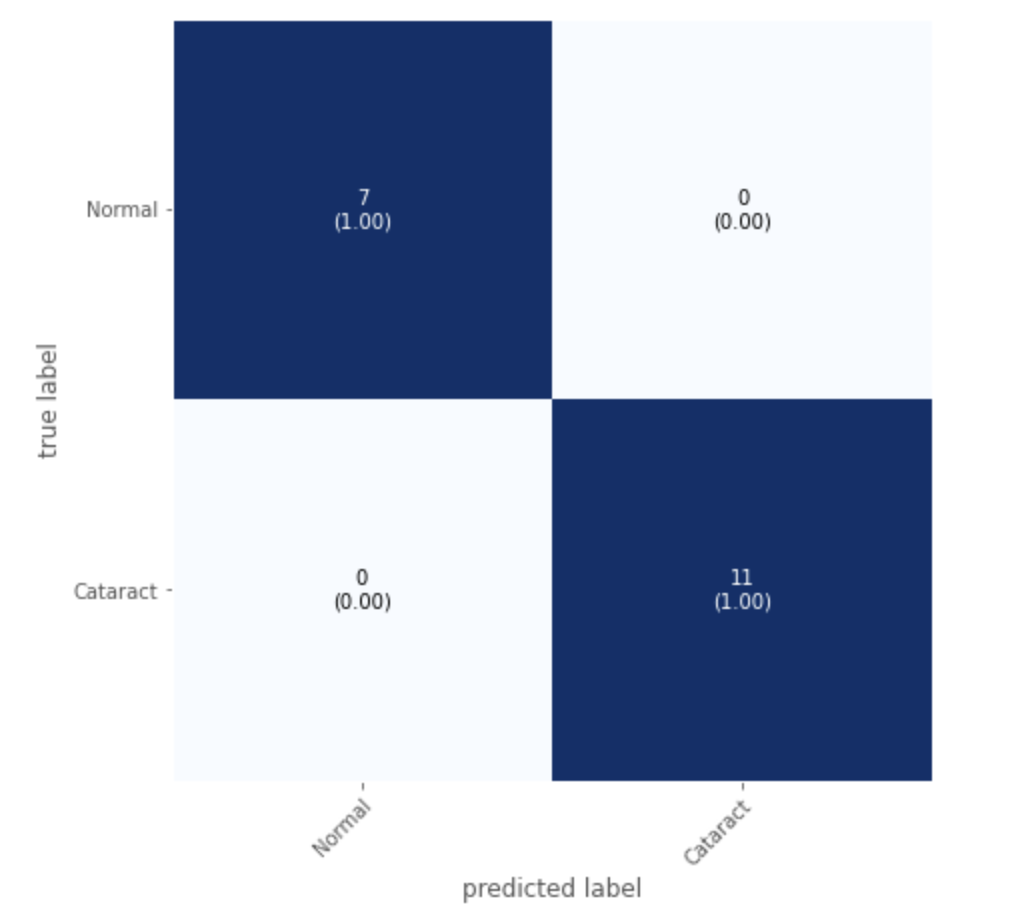
\includegraphics[width=\textwidth]{resnet50_confusion.png}
    \caption{Confusion matrix of ResNet50 model after LBP preprocessing}
    \end{minipage}
\end{figure}


\begin{figure}[htbp]
    \centering
    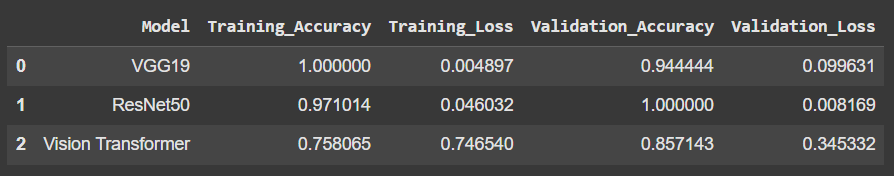
\includegraphics[width=1\textwidth]{image17.png}
    \caption{Comparison table of model metrics after LBP: ResNet50 reached perfect validation accuracy (100\%) with minimal loss (0.008); Vision Transformer showed improved generalization performance.}
    \label{fig:comparison_after_lbp}
\end{figure}

\begin{figure}[htbp]
    \centering
    \begin{minipage}[b]{0.48\textwidth}
    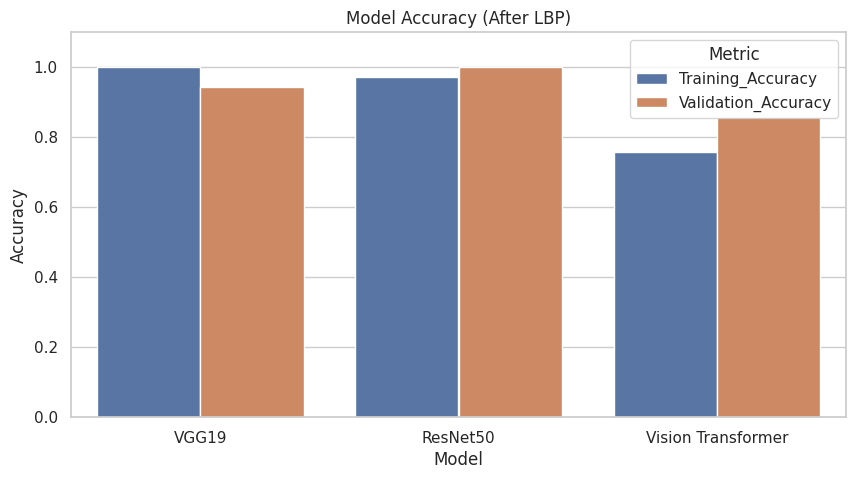
\includegraphics[width=\textwidth]{image19.png}
    
    \caption{Model accuracy after LBP}
    \end{minipage}
    \hfill
    \begin{minipage}[b]{0.48\textwidth}
    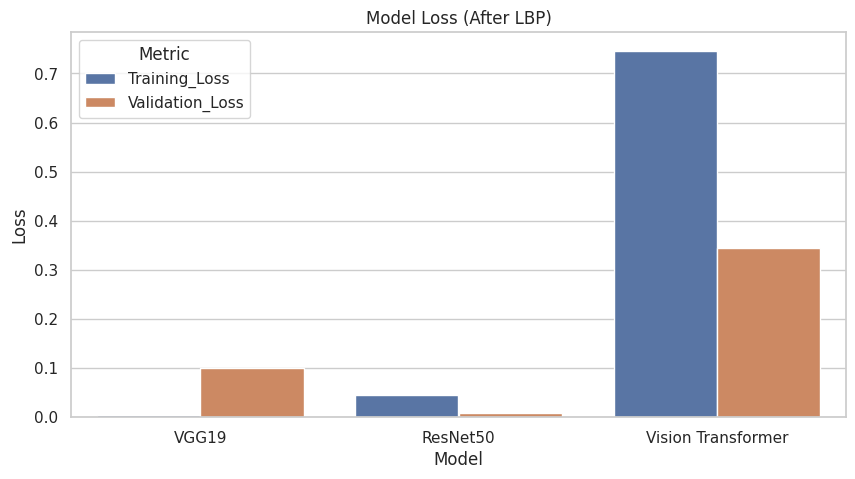
\includegraphics[width=\textwidth]{image20.png}
    \caption{Model loss after LBP}
    \end{minipage}
\end{figure}
\vspace{10cm}
\end{flushleft}
\begin{flushleft}

  \subsection{Comparative visualization of Model Performance With and Without LBP}
  \vspace{1em}

   The comparative visualization of model performance with and without Local Binary Pattern (LBP), as shown in Figures~(\ref{fig:valacc}) and~(\ref{fig:valloss}), shows the impact of LBP on validation accuracy and validation loss of VGG19, ResNet50, and Vision Transformer (ViT), highlighting LBP’s role in enhancing ResNet50 and ViT’s performance while slightly impacting VGG19’s generalization negatively.
   \vspace{1em}

\begin{figure}[htbp]
    \centering
    \begin{minipage}[b]{0.48\textwidth}
    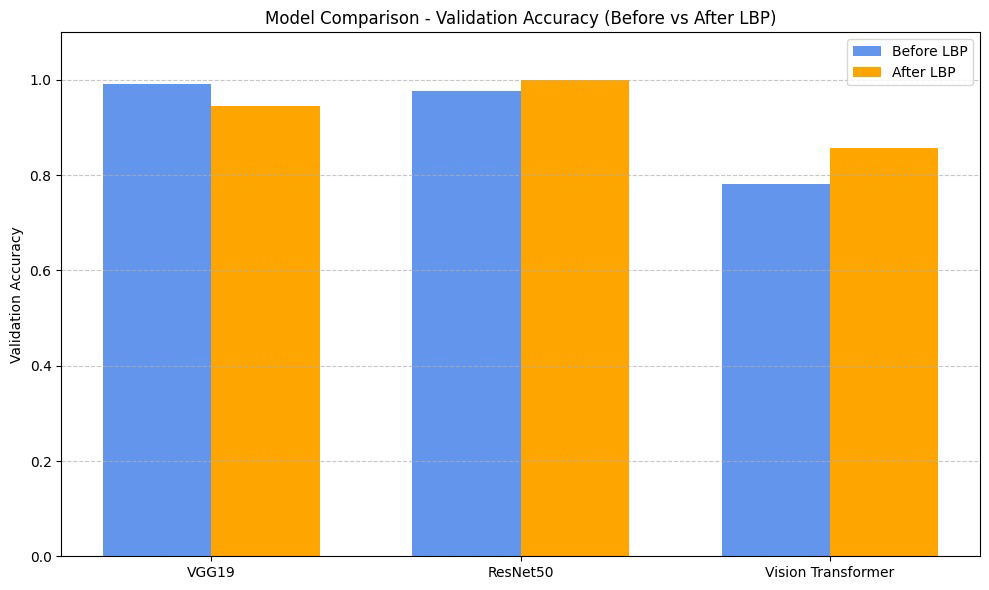
\includegraphics[width=\textwidth]{image21.png}
    \caption{Validation accuracy before vs after LBP for VGG19, ResNet50 and ViT}
    \label{fig:valacc}
    \end{minipage}
    \hfill
    \begin{minipage}[b]{0.48\textwidth}
    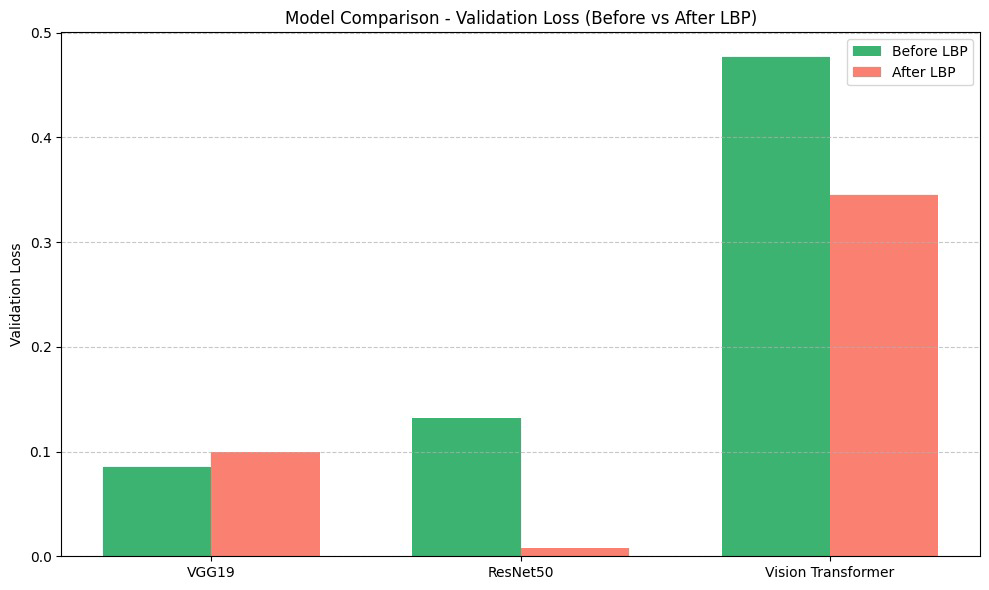
\includegraphics[width=\textwidth]{image22.png}
    \caption{Validation loss before vs after LBP for VGG19, ResNet50 and ViT}
    \label{fig:valloss}
    \end{minipage}
\end{figure}

\end{flushleft}

\begin{flushleft}
    \subsection{Generalization and Overfitting Analysis:}
    \begin{figure}[H]
    \centering
    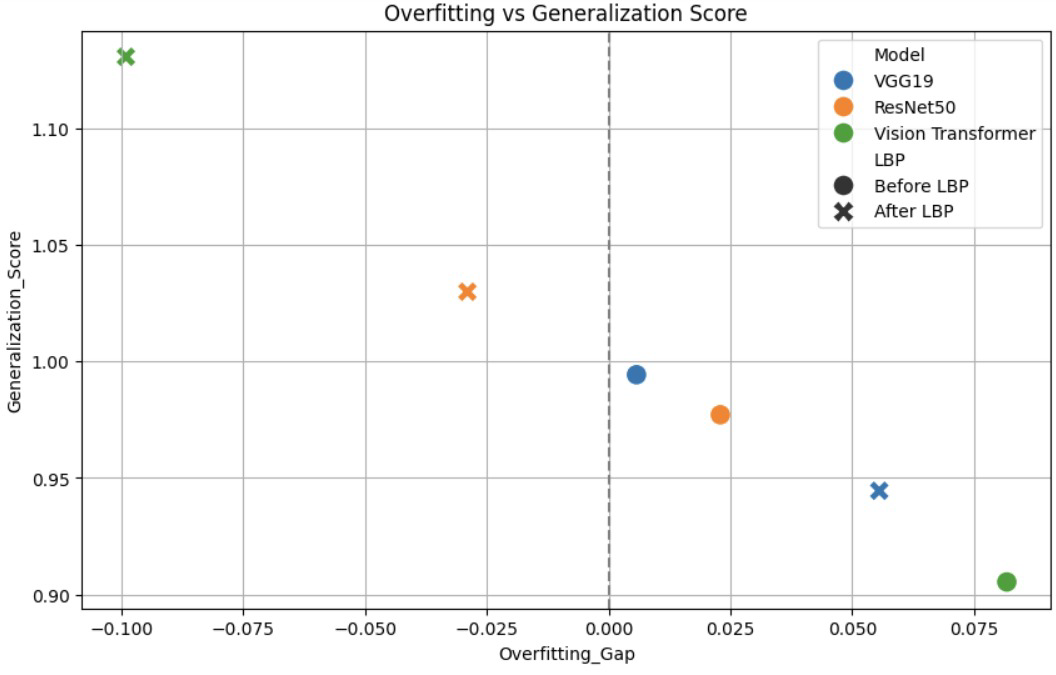
\includegraphics[width=0.7\linewidth]{image23.png}
    \caption{Generalization score vs overfitting gap}
\end{figure}

\begingroup
\sloppy
\begin{equation}
\text{Overfitting Gap (X-axis)} = \text{Training Accuracy} - \text{Validation Accuracy}
\label{eq:overfitting_gap}
\end{equation}

\endgroup

\begin{flushleft}
Overfitting is indicated by positive values, underfitting by negative values, and near-zero values suggest balance. Generalization score is calculated as:
\begin{equation}
\text{Generalization Score (Y-axis)} = \frac{\text{Validation Accuracy}}{\text{Training Accuracy}}
\label{eq:generalization_score}
\end{equation}


For VGG19, the overfitting gap increased slightly from 0.006 to 0.056 after applying LBP, with the generalization score dropping from 0.994 to 0.944, indicating a minor decline in generalization. ResNet50 showed mild overfitting before LBP, with an overfitting gap of 0.0239 and a generalization score of 0.977, however, after LBP, the overfitting gap improved to -0.029, and the generalization score rose to 1.026, reflecting improved generalization. The Vision Transformer exhibited the worst generalization before LBP, with an overfitting gap of 0.0817 and a generalization score of 0.905. After LBP, it achieved an excellent generalization boost, with the overfitting gap improving to -0.098 and the generalization score increasing significantly to 1.126.
\end{flushleft}
\end{flushleft}


\begin{table}[htbp]
\centering
\caption{Comparative Performance Metrics for All the Models With and Without LBP}
\label{tab:lbp_comparison}
\setlength{\tabcolsep}{8pt} % Adjust column padding if needed
\small % makes font smaller for better fit
\begin{tabular}{@{} l l c c c c c c c c @{}}
\toprule
\textbf{Model} & \textbf{LBP} & \textbf{Accuracy} & \textbf{Precision} & \textbf{Recall} & \textbf{F1-Score} & \textbf{Val Acc} & \textbf{Val Loss} \\
\midrule
VGG19     & No  & 0.98  & 0.98  & 0.98  & 0.98 & 0.9908 & 0.0849 \\
ResNet50  & No  & 0.98  & 0.98  & 0.975 & 0.98 & 0.9771 & 0.1315 \\
ViT       & No  & ---   & ---   & ---   & ---   & 0.7816 & 0.4764 \\
VGG19     & Yes & 1.00  & 1.00  & 1.00  & 1.00 & 0.9444   & 0.0996 \\
ResNet50  & Yes & 1.00  & 1.00  & 1.00  & 1.00 & 1.0000   & 0.0082 \\
ViT       & Yes & ---   & ---   & ---   & ---   & 0.8571   & 0.3453 \\
\bottomrule
\end{tabular}
\end{table}



\section{Conclusion}\label{sec:con}
\begin{flushleft}
\justifying
Our study highlights the significant impact of Local Binary Pattern (LBP) preprocessing in improving generalization for deep learning models in binary ocular disease classification (Cataract vs. Normal), with a novel finding that LBP particularly enhances Vision Transformer (ViT) performance, a result not previously reported. We evaluated VGG19, ResNet50, and ViT using transfer learning, with and without LBP. Without LBP, VGG19 led with 99.08\% validation accuracy but showed slight overfitting, ResNet50 hit 100\% training accuracy but only 97.70\% validation accuracy (indicating overfitting), and ViT lagged at 86.33\% training and 78.16\% validation accuracy, suggesting underfitting. With LBP, ResNet50 excelled, achieving 100\% validation accuracy and a low loss of 0.008, while VGG19’s validation accuracy dropped to 94.44\%, increasing overfitting, and ViT improved to 85.71\% validation accuracy, though its training accuracy (75.81\%) still indicated underfitting. These results show that LBP significantly boosts CNN-based models like ResNet50 by enhancing their ability to detect fine-grained patterns in fundus images, while ViT benefits but may need further optimization or larger datasets to fully leverage LBP. Future work could extend this framework to multiclass classification using the ODIR dataset’s eight disease categories, test robustness on diverse cross-institutional datasets, and incorporate explainability tools like SHAP or Grad-CAM to improve interpretability and clinical trust. Additionally, combining CNNs and Transformers in ensemble models could further enhance diagnostic performance through complementary feature learning.
\end{flushleft}

\begin{table}[H]
\centering
\caption{Summary of Model Performance and Observations Before and After LBP}
\label{tab:conclusion_summary}
\resizebox{\textwidth}{!}{%
\begin{tabular}{@{}l p{4.2cm} p{4.2cm} p{4.2cm}@{}}
\toprule
\textbf{Model} & \textbf{Before LBP Observation} & \textbf{After LBP Observation} & \textbf{Conclusion} \\
\midrule
VGG19 & High validation accuracy (99.08\%) with slight overfitting & Validation accuracy dropped (94.44\%), overfitting increased & LBP slightly reduced generalization \\
\addlinespace
ResNet50 & Perfect training accuracy, slight drop in validation (97.70\%) & Perfect validation accuracy (100\%) with low loss & LBP improved generalization significantly \\
\addlinespace
Vision Transformer & Underfit (78.16\% validation accuracy) & Improved validation accuracy (85.71\%) but still underfit & LBP helped, but needs more tuning or data to reduce underfitting \\
\bottomrule
\end{tabular}%
}
\end{table}

% References
\bibliographystyle{plain}
\bibliography{references}

\begin{itemize}
\bibitem{habehh2021mlhealth}
\href{https://doi.org/10.2174/1389202922666210705124359}{
Habehh, H., \& Gohel, S. (2021). Machine Learning in Healthcare. \textit{Current Genomics}, 22(4), 291–300.}

\bibitem{xu2023automatic}
\href{https://doi.org/10.1016/j.compbiomed.2023.107616}{
K. Xu et al., "Automatic detection and differential diagnosis of age-related macular degeneration from color fundus photographs using deep learning with hierarchical vision transformer," \textit{Comput. Biol. Med.}, vol. 167, Dec. 2023, Art. no. 107616. doi: 10.1016/j.compbiomed.2023.107616}

\bibitem{li2023cross}
\href{https://doi.org/10.3390/bioengineering10091100}{
R. Li, Y. Gu, X. Wang, and J. Pan, "A cross-domain weakly supervised diabetic retinopathy lesion identification method based on multiple instance learning and domain adaptation," \textit{Bioengineering}, vol. 10, no. 9, Art. no. 1100, Sep. 2023. doi: 10.3390/bioengineering10091100}

\bibitem{singh2024novel}
\href{https://doi.org/10.1007/s11042-023-17081-3}{
L. K. Singh et al., "A novel hybridized feature selection strategy for the effective prediction of glaucoma in retinal fundus images," \textit{Multimed Tools Appl}, vol. 83, pp. 46087–46159, 2024. doi: 10.1007/s11042-023-17081-3}

\bibitem{aktas2024diffusion}
\href{https://doi.org/10.1007/s13042-024-02485-w}{
B. Aktas et al., "Diffusion-based data augmentation methodology for improved performance in ocular disease diagnosis using retinography images," \textit{Int. J. Mach. Learn. \& Cyber.}, 2024. doi: 10.1007/s13042-024-02485-w}

\bibitem{yassin2023fundus}
\href{https://doi.org/10.47760/ijcsmc.2023.v12i05.006}
{N. I. R. Yassin, "Fundus Images Classification of Diabetic Retinopathy using MobileNetV2," \textit{Int. J. Comput. Sci. Mob. Comput.}, vol. 12, no. 5, pp. 54–63, May 2023.}

\bibitem{guergueb2021ocular}
\href{https://doi.org/10.1109/EMBC46164.2021.9629763}{%
Takfarines Guergueb and Moulay A. Akhloufi, 
"Ocular Diseases Detection using Recent Deep Learning Techniques," 
\textit{Proceedings of the 2021 Annual International Conference of the IEEE Engineering in Medicine and Biology Society (EMBC)}, 
pp. 3336--3339, Nov. 2021. DOI: 10.1109/EMBC46164.2021.9629763}


\bibitem{ye2024ocular}
\href{https://doi.org/10.1007/s40123-024-01009-7}
{X. Ye et al., "Ocular disease detection with deep learning (fine-grained image categorization) applied to ocular B-scan ultrasound images," \textit{Ophthalmol. Ther.}, vol. 13, pp. 2645–2659, Aug. 2024.}

\bibitem{du2024recognition}
\href{https://doi.org/10.1186/s12880-023-01176-2}
{F. Du et al., "Recognition of eye diseases based on deep neural networks for transfer learning and improved D-S evidence theory," \textit{BMC Med. Imaging}, vol. 24, no. 19, 2024.}

\bibitem{halapathirana2023lbp}
\href{https://aihalapathirana.medium.com/understanding-the-local-binary-pattern-lbp-a-powerful-method-for-texture-analysis-in-computer-4fb55b3ed8b8}
{A. Halapathirana, "Understanding the Local Binary Pattern (LBP): A Powerful Method for Texture Analysis in Computer Vision," \textit{Medium}, Jul. 25, 2023.}

\bibitem{odir5k}
\href{https://www.kaggle.com/datasets/andrewmvd/ocular-disease-recognition-odir5k}
{Andrew Mvd., "Ocular Disease Recognition (ODIR-5K) Dataset," 2019. Available on Kaggle.}

\bibitem{resnet50medium}
\href{https://medium.com/@nitishkundu1993/exploring-resnet50-an-in-depth-look-at-the-model-architecture-and-code-implementation-d8d8fa67e46f}
{Kundu, N., "Exploring ResNet50: An In-depth Look at the Model Architecture and Code Implementation," \textit{Medium}, 2023.}

\bibitem{resnet}
\href{https://doi.org/10.1109/CVPR.2016.90}{
He, K., Zhang, X., Ren, S., \& Sun, J. (2015). Deep Residual Learning for Image Recognition. Proceedings of the IEEE Conference on Computer Vision and Pattern Recognition (CVPR), 770-778.}

\bibitem{vggmedium}
\href{https://medium.com/@siddheshb008/vgg-net-architecture-explained-71179310050f}{
Bhoite, S. (2020). \textit{VGG Net Architecture Explained}. Medium.}

\bibitem{hu2024}
\href{https://example.com/deep-learning-vgg19}{
Hu, J. (2024). Deep Learning in Image Classification: Evaluating VGG19's Performance on Complex Visual Data.}

\bibitem{rahmani1996baltimore}
\href{https://doi.org/10.1016/S0161-6420(96)30435-1}{
Rahmani, B., Tielsch, J. M., Katz, J., Gottsch, J., Quigley, H., Javitt, J., \& Sommer, A. (1996). The cause-specific prevalence of visual impairment in an urban population: The Baltimore Eye Survey. \textit{Ophthalmology}, 103(11), 1721–1726.}


\bibitem{vitmedium}
\href{https://medium.com/@hansahettiarachchi/unveiling-vision-transformers-revolutionizing-computer-vision-beyond-convolution-c410110ef061}{
Hettiarachchi, H. (2023). \textit{Unveiling Vision Transformers: Revolutionizing Computer Vision Beyond Convolution}. Medium.}




\bibitem{whovision2019}
\href{https://www.who.int/publications/i/item/world-report-on-vision}{
World Health Organization, \textit{World Report on Vision}. Geneva: World Health Organization, 2019. [Online].}

\bibitem{oculardiseasePMC}
\href{https://www.ncbi.nlm.nih.gov/pmc/articles/PMC9071974/}{
Chaki, J., Gan, K. S., Dey, N., Das, A., \& Tavares, J. M. R. S. (2022). \textit{Machine Learning and AI-Based Approaches for Ocular Disease Detection: A Comprehensive Review}. Diagnostics, 12(5), 1084.}

\bibitem{prajapati2023retinal}
\href{https://doi.org/10.1109/ICCECE51049.2023.10085191}{
M. Prajapati, S. K. Baliarsingh, J. Hota, S. Das, et al., "Retinal and Semantic Segmentation of Diabetic Retinopathy Images Using MobileNetV3," in Proceedings of ICCECE, January 2023.}

\bibitem{patel2022spatial}
\href{http://dx.doi.org/10.14569/IJACSA.2022.0130519}{
Sanskruti Patel, Rachana Patel, Nilay Ganatra and Atul Patel, “Spatial Feature Fusion for Biomedical Image Classification based on Ensemble Deep CNN and Transfer Learning,” \textit{International Journal of Advanced Computer Science and Applications (IJACSA)}, 13(5), 2022.}

\bibitem{armstrong2014eye}
\href{https://doi.org/10.1016/B978-0-12-401717-7.00001-0}{
Armstrong, R. A., \& Cubbidge, R. P. (2014). Chapter 1 - The eye and vision: An overview. In R. Rosen \& C. S. McCabe (Eds.), \textit{Visually Memorable Neuroscience} (pp. 1–17). Academic Press.}

\bibitem{weni2021cataract}
\href{https://doi.org/10.22146/ijccs.61882}{
Weni, I., Utomo, P. E. P., Hutabarat, B. F., \& Alfalah, M. (2021). Detection of Cataract Based on Image Features Using Convolutional Neural Networks. \textit{Indonesian Journal of Computing and Cybernetics Systems}, 15(1), 75–84.}


\end{itemize}

\end{document}


\begin{figure}[ht]
    \centering
    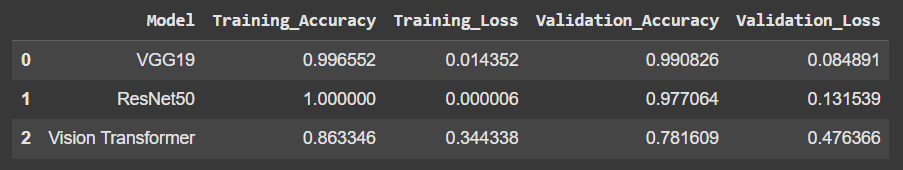
\includegraphics[width=0.49\linewidth]{image12.png}
    \caption{Comparison Table for all the models before
LBP}
    \label{fig:enter-label}
\end{figure}
\begin{figure}[ht]
    \centering
    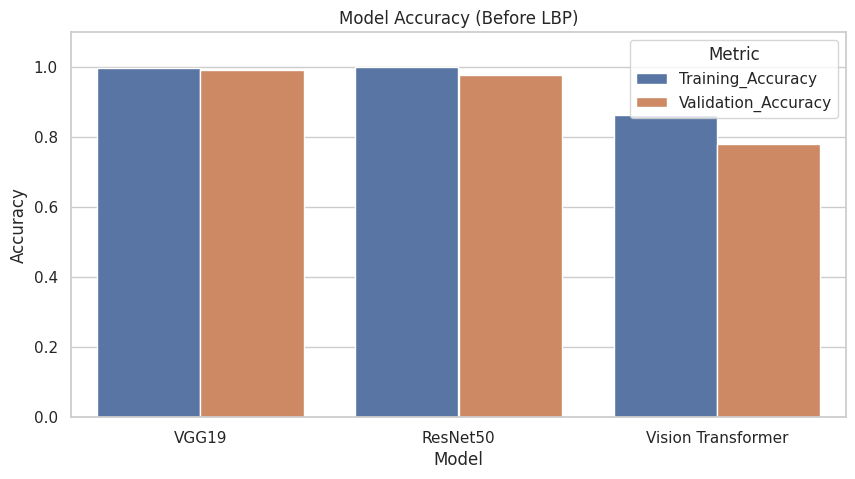
\includegraphics[width=0.49\linewidth]{image13.png}
    \caption{Model accuracy before LBP}
    \label{fig:enter-label}
\end{figure}

\subsubsection{Title}
From the results shown in Table 5...

% Table Example
\begin{table}[h]
    \centering
    \begin{tabular}{lllrrr}
        \toprule
        Testing Data & Sources & Hardness & Rule type-1 & Rule type-2 & Rule type-3\\
        \midrule
        Sinica & Balanced corpus & Moderate & 92.97 & 94.84 & 96.25 \\
        Sinorama & Magazine & Difficult & 90.01 & 91.65 & 93.91\\
        Textbook & Elementary school & Easy & 93.65 & 95.64 & 96.81 \\
        \bottomrule
    \end{tabular}
    \caption{The 50-best oracle performances from the different grammars.}
\end{table}


\begin{figure}
    \centering
    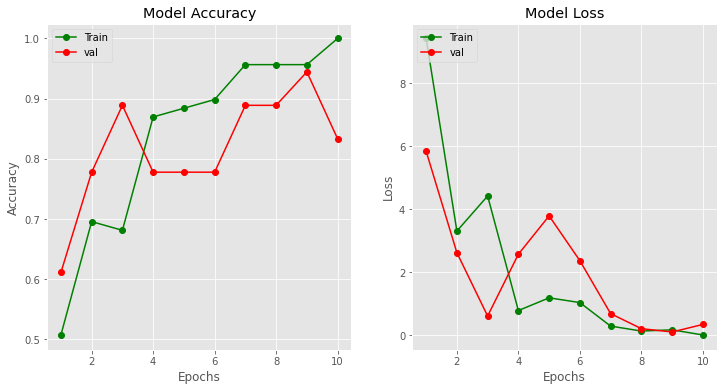
\includegraphics[width=0.5\linewidth]{image14.png}
    \caption{VGG - 19}
    \label{fig:enter-label}
\end{figure}

\begin{figure}
    \centering
    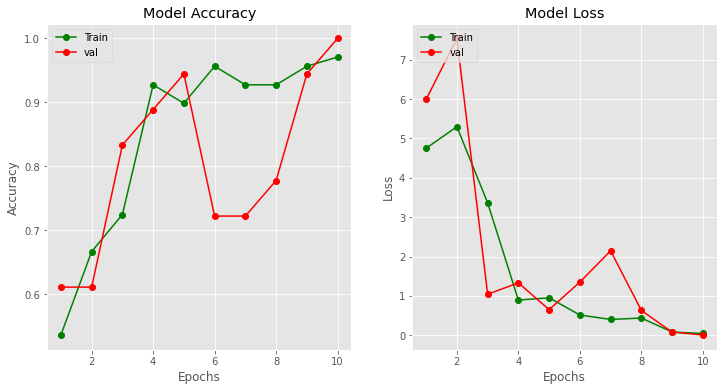
\includegraphics[width=0.5\linewidth]{image15.png}
    \caption{ResNet50}
    \label{fig:enter-label}
\end{figure}

\section*{Acknowledgments}
This research was supported in part by National Science Council under Grant NSC 95-2422-H-001-008- and National Digital Archives Program Grant 95-0210-29-戊-13-09-00-2.


\begin{figure}[ht]
    \centering
    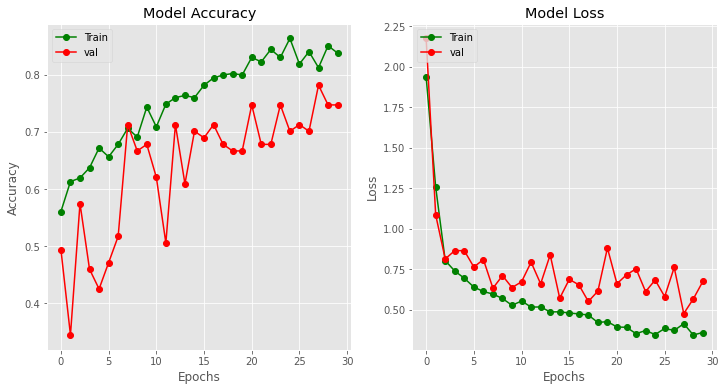
\includegraphics[width=0.595\linewidth]{image11.png}
    \caption{Vision Transformer}
    \label{fig:enter-label}
\end{figure}

\begin{figure}
    \centering
    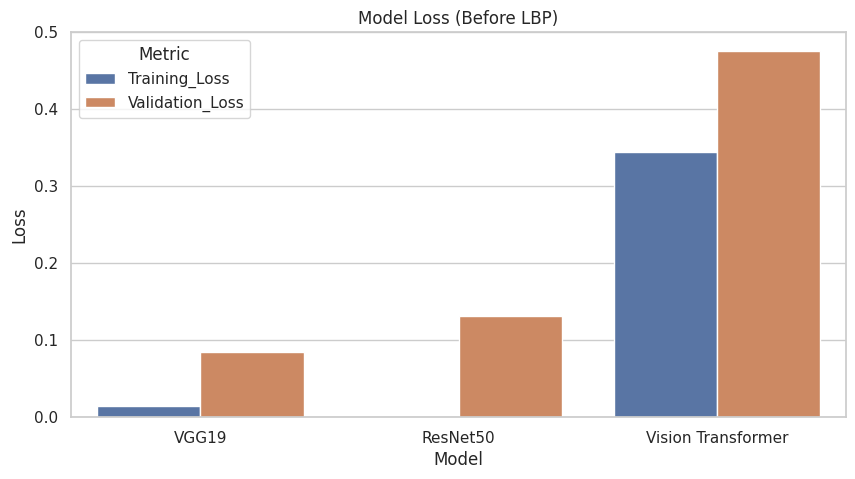
\includegraphics[width=0.5\linewidth]{image18.png}
    \caption{Model loss before LBP}
    \label{fig:enter-label}
\end{figure}

\begin{figure}
    \centering
    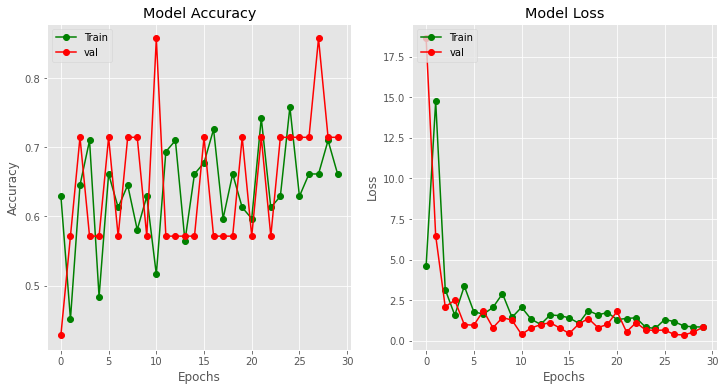
\includegraphics[width=0.595\linewidth]{image16.png}
    \caption{Vision Transformer}
    \label{fig:enter-label}
\end{figure}
\begin{figure}
    \centering
    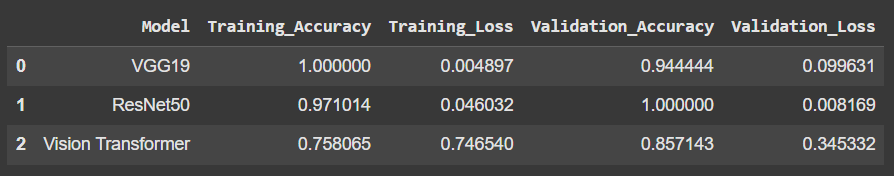
\includegraphics[width=0.5\linewidth]{image17.png}
    \caption{Comparison table for all the models after
LBP. The table shows that ResNet50 performs very well
with validation accuracy (100\%) and low loss (0.008),
while Vision Transformer underfit with 75.8\% training and
85.7\% validation accuracy.}
    \label{fig:enter-label}
\end{figure}

